\documentclass[minf,twoside,singlespacing,parskip,frontabs,notimes,11pt]{infthesis} 

\usepackage{url}
\usepackage{graphicx}
\usepackage{subfig}
\usepackage{wrapfig}

%\usepackage{biblatex}
%\usepackage[xetex]{graphicx}
%
%\usepackage{fontspec,xunicode}
%
%\defaultfontfeatures{Mapping=tex-text,Scale=MatchLowercase}
%\setmainfont[Scale=.95]{Georgia}
%\setmonofont{Georgia}


\usepackage{amsmath}
\newcommand{\BigO}[1]{\ensuremath{\operatorname{O}\bigl(#1\bigr)}}

\usepackage{listings}
\usepackage{color}

\definecolor{dkgreen}{rgb}{0,0.6,0}
\definecolor{gray}{rgb}{0.5,0.5,0.5}
\definecolor{mauve}{rgb}{0.58,0,0.82}

\lstset{frame=tb,
  language=Python,
  aboveskip=3mm,
  belowskip=3mm,
  showstringspaces=false,
  columns=flexible,
  basicstyle={\small\ttfamily},
  numbers=left,
  numberstyle=\tiny\color{gray},
  keywordstyle=\color{blue},
  commentstyle=\color{dkgreen},
  stringstyle=\color{mauve},
  breaklines=true,
  breakatwhitespace=true
  tabsize=4
}

\begin{document}
\title{Modelling search volumes as a dynamic system responding to external events}

\author{Stefan Sabev}

\course{Master of Informatics}
\project{{\bf MInf Project (Part 1) Report}}

\date{\today}

\abstract{
It is well known that some events might spark people's interest to fly to different destinations. In particular news events or sports events can quite easily make people search for a specific destination - for example the Champions League Quarter final draw increased the number of flight searches from Glasgow to Spain by a factor of 6.\\
The goal of this project is to prove that by taking social media into account, one can build a better model to predict flight search volumes. \\
For this project we have collected vast amounts of Twitter data. With this dataset and the flight search dataset provided by Skyscanner it was possible to build a model that predicts flight search demand based on what's happening on Twitter. This is a novel approach to predicting flight search volumes utilising the vastness of Social data available. \\
The potential applications of this are generic prediction of flight search volumes, predicting new events for better marketing and also anomaly detection in traffic caused by events.
}

\maketitle

\section*{Acknowledgements}

First of all, I'd like to thank Charles Sutton for supervising this project. All of his guidance made this possible.\\
\\
A big thank you also goes to Ewan Nicolson for all of his help with the project.

\tableofcontents

\pagenumbering{arabic}

\chapter{Introduction and background}

\section{Introduction}

In this project we will make the first attempt ever to incorporate social media data into flight searches prediction. As a consequence of that we can measure to what extent social media impacts online travel. We will show that using Twitter data in particular, which has been collected since the 24th of September 2013 (550 GB, 650 million tweets) we can employ text mining and use the Twitter data in a model that will predict flight search volumes. With this model we will be able to see the upward and downward shifts in demand caused by events. With Natural Language Processing (NLP) we will hopefully gain better understanding on how to predict demand and therefore this could be useful not just to flight search companies, but also to airlines and airports. 


There aren't that many flight search companies with the global outreach required to collect and aggregate massive volumes of flight search data. And there are even fewer ones that are making some or the whole of their datasets available for research. When you consider that and the fact that online travel is a niche area in itself, one starts to understand why research of this kind would have been quite hard if not impossible to do up until this date. However as some of those companies grow, they are trying to employ more sophisticated ways of predicting demand and as a result of that plan their hardware capacity better or just to improve their revenue forecasting. With the rise of social media, the next logical step would be to start exploring different ways of adding exogenous factors such as data extracted from Twitter into their models to better their prediction. 


It will be impossible not to say anything about Skyscanner, since they have kindly provided the flight search data, which I am using in this project. \footnote{\textbf{Dislaimer}: I am an employee of the company and have been working there since 2011} It's an Edinburgh-based company with offices around the whole world. It the past years it has been slowly, but surely positioning itself as a leader in online travel search. It is in a phase of rapid growth. Doubling in size and valuation for the past couple of years helped secure an investment from Sequoia Capital \cite{seqcap}.  


Due to the fact it processes billions of user searches on a monthly basis it is quite important to be able to predict future searches, because there could be a knock-on effect on the capacity, the website performance and the costs in general. This has made Skyscanner transform from a flight search company into a data-driven travel company. Many companies are realising lately that with ``Big Data" comes big responsibility -- you need to get the maximum value out of your data rather than just store it on disk. In order to utilise all of it Skyscanner have developed and deployed a lot of in-house algorithms for anomaly detection and forecasting all of their Key Performance Indicator (KPIs). However there are still some things that you can't predict from just looking at past data and learning from it.


This particular project was spurred after a discussion that social media could be harnessed to produce some form of aggregated counts that will allow us to see whether there are going to be any expected spikes to any destinations -- cities and countries with an airport. Of course that will not be a ``one size fits all" approach, since some places such as London, Paris and New York will see very high steady number of search volumes to them. The destinations that are more likely to be better predicted by the model with Twitter are the ones that are not constant all year round -- Ibiza, Alicante, Dubrovnik and many others. Those destinations have a particular type of very well expressed seasonality with spikes around holidays and some events, which the Twitter data should hopefully capture.


Initially I had to mine the vast quantities of Twitter data in a particular way (described in the  Chapter \ref{chap:method}: Methodology) and then take the numbers aggregated by day to produce what we will call in this dissertation the ``Twitter counts" for a particular destination or overall. The in-house model for predicting the searches will hopefully be beaten by the new improved model with Twitter factored in. The approach described here could be used to develop a system that monitors one or more social streams and use the mined and aggregated data as an additional feature in a system of models for predicting the future based on past data, but also taking Twitter into account.


In the first part of the project I have decided to be as pragmatic as possible and explored the most practical of all potential uses - predicting search volumes for every city or country that has been mentioned on Twitter with the counts and a list of features that are automatically extracted from the public stream. Based on the aggregated numbers and the historical data we train a model which is then used to predict the volumes for the future and evaluate them.


When the project is extended to be a more real-time system in its second phase, I expect that with the help of some TDT the potential applications of the work here are going to be used in several areas. In theory, one can easily plug in to a social network public stream and monitor what is happening, what is trending and as soon as something relevant is seen -- either an event in a different country/city or something else -- one can action in a multitude of ways:


\begin{itemize}
\item "X is happening, why not fly there to see it?"
\item The system can be developed further to monitor multiple source of social media in real time for potential spikes in traffic. That is very useful, because in 2011 the website was mentioned on an Italian TV show and because of the boom in traffic from Italy the website was down for half an hour. 
\item If cross-referenced with a capable Customer Relationship Management system you could use the methods described in this project and the results as a data source for a real time marketing solution.
\end{itemize}


%The incredible breadth, the opportunity to work with big datasets and the fact that I could work on something novel were the main reasons that made me pick this particular topic for research in my project. It's a very interesting mixture of Machine Learning and Natural language processing. It has also presented a brilliant opportunity to learn how real life ML and NLP can be used and applied to a big dataset and what are the potential benefits of doing so. Of course, it's worth mentioning that there is also the practical aspect of building a model that could be used to power a system for predicting search volumes and also anomaly detections with some slight tweaks. 


\textbf{Note} - All the aggregated datasets are made available in the GitHub repository \cite{code}.  The full Twitter dataset will be made available on request. Of course because of confidentiality I can't publish the dataset which has the Skyscanner searches, since that will break my employee code of conduct. Instead, in order to present the results here, I have anonymised the search volumes by normalising as described in the methodology. 


\section{Background and discussion of related work}


With millions and some with billions of users, social networks are becoming an increasingly more important part of our lives. A big proportion of people use it as their primary way of communicating with the outside world - people will ``tweet" about anything, post to Facebook, check in on FourSquare, Instagram their food and so on. We have become perfectly fine with externalising our lives and posting every minute detail online and thusly making it available to everyone else. 
Of course, there are always exceptions. After all 82\% of the world's population are not on Facebook, but the 1.31 billion monthly active users are all using it \cite{FBStats}. Not all of them are avid users and post all of their pictures to it, but a big proportion is \cite{FBStats}. With this amount of data on one's behaviour, life patterns and activities, companies can build a very good understanding of every individual and potential customer.


As with any other network -- be it TV, radio, newspaper -- there are always going to be some who are trying their best to commercialise and benefit from it in some way. Since people are willing to share so much information about themselves online, there are terabytes of data being generated every day on what people did, what things they tweeted about, their latest pictures, what they bought, etc. As we are entering the ``Big Data" age every company is trying to turn its data into a product or simply establish itself as the leading data supplier for a particular market. Due to the vastness, velocity and volume of the data that these social networks generate they have sprung an entirely new eco-system of their own -- companies are now plugging into Twitter, Facebook and all the other networks to figure out everything they can about you. Everyone is now talking about ``sentiment analysis" in social media for brands, targeting particular demographics with ads on Facebook, promoting tweets, segmenting customers into different groups and selling their data to marketers.


A particularly interesting one of the new generation social networks is Twitter. With a base of 190+ million active users \cite{TwitStat} it has slowly but surely become one of the most prominent sources of information and news on the web. It's previously beaten traditional news sources in delivering news on numerous occasions by a few minutes. For instance when the Los Angeles earthquake happened in 2008 \cite{TwitterNewsWire} Twitter reacted seconds afterwards, while traditional media took 4 minutes. They have their public streams opened up to developers and researchers as well, which is a fantastic opportunity to mine this dataset for valuable information. There are plenty of articles on the internet on what people have done with it - demographics research, predicting flu outbreaks, etc \cite{TwitterResearch}.  After researching the topic, I found that the School of Informatics already has done a lot of work on harnessing social media for various applications. Sasa Petrovic and Miles Osborne have looked into using paraphrases in Twitter \cite{Miles1} and have also tried predicting deleted Twitter messages \cite{Miles2}. After more careful investigation I found perhaps the most innovative use of all in Sasa Petrovic's PhD thesis  -- ``Real-time event detection in massive streams" \cite{Petrovic2012}.


After reading Sasa's thesis \cite{Petrovic2012} I investigated the option to incorporate Topic Detection and Tracking and First News Detection into my project.  However after careful investigation into the complexity of TDT, I decided that I will postpone that until 2nd part of the project, because of more pressing matters -- familiarising myself with the datasets and seeing how are they are correlated, so I could implement more sophisticated filtering and try out the simplest ways of predicting flight search volumes.


The great Niels Bohr has said: ``Predicting is hard, especially about the future''.  Add a noisy channel as a source and things are only made worse. There have been several attempts to predict something based on Twitter: stock markets \cite{twitstock},  flu outbreaks \cite{twitflu}, results for the NFL \cite{twitnfl} and poll results \cite{twitpoll} being the most prominent published papers. I will analyse them in more detail and provide a summary of what was achieved and what methods were used in them.


In order to predict the stock markets \cite{twitstock}, Johan Bollen and Huina Mao try to use the cutting edge of the real-time twitter data in order to classify the overall mood and from that to predict whether the DIJA \cite{dija} is going to go up or down. In order to achieve it they use OpinionFinder (OF) \cite{opfind}, which can measure opinion classifying it into negative or positive. To capture the complexity of human moods, they created their own system called GPOMS, which can capture up to 6 states. 
In order to make the OF and GPMOS time series comparable, they used their z-scores. They have proven that the GPOMS values are more descriptive of public moods than the OF binary sentiment. However correlation does not imply causation and in order to check whether there is any they use the Granger causality analysis \cite{granger}. It rests on the assumption that if X causes Y then changes in X will systematically occur before changes in Y. However in this case they are not testing whether there is actual causation, but if there is predictive information in the public mood time series that can describe the time deltas in DIJA. Out of all the different mood values Calm has the highest predictive value. After determining that there is definitely a gain in using the Calm values to predict the DIJA delta they use a Self-Organising Fuzzy Neural Network (SOFNN) \cite{sofnn}, which is a five-layer hybrid neural network, which with the ability to organise its neurones during the learning process. After tuning and predicting the values on their dataset, they confirmed that Calm has the best predictive value. 

However, in their discussion they not that they are not really filtering their users on any particular geographical, language or cultural level. In this project, we have only taken \emph{tweets} from the United Kingdom, which allows us to try to predict where people from the UK want to fly to. As far as their methods are concerned, working with Neural networks is certainly one of the options that I'd like to investigate next year because of the additional overhead of training, fine tuning and possibly implementing it myself.


On the other hand you can do simpler things when you are trying to predict public opinion on a certain topic \cite{twitpoll}. The authors make a strong argument that using Twitter you can replace the expensive time inefficient polls. They use public sentiment in order to predict ups and downs in the consumer confidence rating. In order to remove any massive outliers caused by the volatile nature of public sentiment they use something they call "Moving average aggregate sentiment", which smoothens out the daily variations. For the classification and prediction they use a Linear Least-Squares model with a lag hyper parameter. The hyper parameter is a good idea for my project and it's certainly a very good option to explore, because sometimes the public might not go out and search flights straight away, but instead do it the next day. That is certainly something that should be considered when building the models later.


Of course Twitter can be used to predict other things with some success -- NFL games \cite{twitnfl} or general state of public health \cite{twitflu}.  In Sinha et al \cite{twitnfl} the authors have used Canonical correlation analysis (CCA) to combine the Twitter features with the statistical game features and to maximise the correlation of the combined features. However even with the more sophisticated CCA and combinations of features, taking Twitter unigrams still perform better than the combined features, which is very surprising. With all of those experiments, their methods still gets only about 50\% prediction accuracy when predicting the winner, which is equivalent to a coin toss. 

In Paul and Dredze \cite{twitflu} the data gathered from Twitter is used to paint a picture of public health in the US. Since a big proportion of the users tweet daily \cite{TwitStat} that allows to perform an in-depth analysis of what is happening around the country. They make the hypothesis that Twitter can be used for more than simple influenza tracking and one can actually analyse the bigger picture with the data collected from it. In order to model the diseases they use a technique called Ailment Topic Aspect Model, which build on top of Latent Dirichlet Allocation \cite{lda}. With that they were able to track flu in the US and when correlated with the health data their ATAM+ model achieved ? coefficient of 0.958. The data is split geographically and over time. As a consequence the authors find a lot of interesting things, which prove that Twitter can definitely be used to paint a picture of what the health of the nation looks. The limitations of the social network are discussed in detail as well. Due to geocoding limitations, they couldn't provide a more specified per user analysis, but overall the correlations in the paper are astonishing and show the breadth that Twitter data gives. 


In the aforementioned papers I have shown the different ways in which Twitter could be used to predict something about the future. Since people are inclined to post a lot of information on it, why wouldn't we be able to do something something specific in a niche area like predicting search volumes or anything to do with the airline industry?

The only thing that has been researched in the online travel sector is what is the optimal time to book an airline flight \cite{Hamletkdd03,ijcai}.  In order to do it a lot of factors have to be considered, because human action can cause massive shifts in prices very easily. 
Both of the aforementioned papers are using small sets of data which aim to predict what is the optimal time to book. What is written there is the other part of the puzzle - when should you book, but in this particular project we are more interested in when \textit{are} people looking for flights.

\section{Outline}

The Methodology can be found in Chapter \ref{chap:method}, split by all the main subtasks that had to be carried out. The subtasks are described in detail and each one of the sections includes an overview of what was done, how it was done and what difficulties were encountered and how I overcame them. 


Chapter \ref{chap:model} explains what are the Machine Learning (ML) models used to carry out the work for this project. The lack of previous work in the area left with only one candidate to use as a baseline -- the in-house model developed at Skyscanner. All of the models are outlined and presented in detail with some justifications on why they are used. 


In Chapter \ref{chap:results} you can find the discussion and presentation of all the results obtained while evaluating my models. The discussions is backed up by tables and figures in order to present the data to the reader in the most natural way.


In Chapter \ref{chap:future-work} I have discussed all the possible avenues for future work split by the different areas. They are a discussions on the improvements to be made with Machine Learning, Natural Language Processing and some of the things that Skyscanner could do to incorporate this into their operations. 

\section{Contributions}


Here is a brief summary of the main contributions of this project.

\begin{itemize}
\item \textbf{I developed a scalable system for storing, analysing, exploring and visualising the data.}
\item \textbf{In this work I have also explored what effects social media has on online travel -- what causes shifts in demand.}
\item \textbf{I suggested, explored and implemented a novel way of predicting flight search volumes with taking exogenous factors into account.}
\item \textbf{As a result of my models I have managed to improve overall prediction of flight search volumes by 5\% while capturing the trends in previous demand and spikes caused by events such as the Winter olympics and the riots in Ukraine.} 
\end{itemize}







\chapter{Methodology}
\label{chap:method}

This problem is not something that has researched before as I have mentioned previously. The lack of previous work and little to none understanding of how to approach it gave me a lot of room to manoeuvre, but it was also very hard to see whether the project is on the right track and whether a right track exists at all.

The overall plan for the first phrase of the project is:
\begin{enumerate}
\item Create an extensible and modular toolset that will allow me to do all of the below-mentioned.
\item Collect data from the Twitter API and the Skyscanner database. 
\item Process the data and convert it to time series.
\item Explore the correlation between the time series from the two datasets
\item Cleanse all the problematic elements by either backfilling where possible or by removing them.
\item Extract the features for the multi feature models.
\end{enumerate}

Each section in this chapter is an in-depth explanation on every one of the afore-mentioned bullets. 

Due to the open ended nature of the project it is not very restrictive. There was a lot do -- after collecting the data I had to explore both of the datasets (described in more detail in Section 2.1). Since that is quite a fuzzy term I wanted to see what information both of them hold and what I can extract. As far as the searches dataset was concerned, since I have been an employee of Skyscanner for some time, I knew exactly what the data is, what it means and I could spot when a number just felt wrong. That was really good, because it did not add any additional overhead and it meant that the Skyscanner dataset did not require any extra effort from me. 


Twitter on the other hand was a challenge. Performing any exploratory analysis on the data was far from trivial, just because of the sheer size. The Sample stream (1\% of all tweets) \cite{samplestream} that I used is giving around 6 GB of data a day, which is not small by any means. With some filtering and picking all the relevant attributes, I decreased the volume down to 3.5 GB daily. I have described in detail the attributes I picked for this project section in Section \ref{sec:dc}. The remaining data equates to half of the original input. As of the time of writing I have gathered 550 GB of data in total. They contain the staggering 650 million tweets. The data has been collected continuously since the 24th of September 2013. 


Dealing with data of this size is not an issue one encounters every day, therefore I had to be very careful of how I design and structure my system. I also had to make sure it is as robust as possible and it is not going to buckle under the volumes of data coming in for processing.


The implication of the data size was that it I now had set of challenges imposed on me.  The success of the project very much depended on how I tackle them:
\begin{enumerate}
\item How do I traverse the data in an efficient and clever manner without overdoing myself or performing unnecessary computation? That meant that I needed to store all the processed data in a way that it's easy to add the data as it comes.
\item What are the appropriate data structures in which I can hold the data, so they are easily transferable onto other parts of my system? What would the data flow be from collection to preparation and then to the models?
\item How do I build a scalable and performant system for data analysis of the tweets, that will allow me to perform experiments in an easy and reproducible fashion?
\end{enumerate}


All of these challenges resulted in me spending at least a 100 hours in designing, building and testing the system that performs all of the computation. All of the code can be found in the code repository on GitHub \cite{code}. The codebase includes separate classes which allow filtering of the data, processing, converting to time series, combining the two datasets together and then performing the regression models on them afterwards. 


In the first set of single Twitter feature models we are using just the Twitter count time series and the searches time series. The 2nd iteration of MultiFeatureTwitter models extracts all the possible words, which it then uses as separate features. In order to cater for that I have created separate classes for the feature extraction task, which is perhaps the most intensive one of them all, hence for the feature extraction I've taken the top 80 destinations + Ukraine because of the recent political and social unrest and North Korea, because of the baffling positive correlation, which is shown in Figure 2.3d.

Taking those expanded feature sets is possible because of the data filtering I perform. That enables to shrink the 500GB dataset into a smaller working dataset of around 50 GBs, which is residing on a local SSD enabling very fast processing and aggregation. 


In this Chapter I describe in detail every one of the main parts of the system. I went from just gathering data to a full system for analysis and visualisation of Twitter data and here I describe all of the big problems I encountered and how I solved them.


\section{Data collection}
\label{sec:dc}


The first and most important step to any Machine Learning project is to collect all the data you can and most importantly the data you need. In my case I had two different sets I had to work with - the data flowing in from the Twitter Public Stream and the search data coming in from Skyscanner. As said previously the data from Skyscanner didn't need any additional work in terms of familiarising myself, because I could easily pull it out with a SQL script and give myself all the necessary aggregations without any problem. 

\begin{table}[h]
\begin{center}
\begin{tabular}{ l | r }
\textbf{Date} & \textbf{Searches}\\
\hline
2013-09-25 &  X \\
2013-09-26 &  Y \\
2013-09-27 &  Z \\
\end{tabular}
\end{center}
\caption{Skyscanner searches time series for a city/country.}
\label{ssearches}
\end{table}



The data obtained from all the SQL querying was the searches time series for 2403 destinations. Those destinations are all the cities with an airports and countries that you can fly to. The time series were stored in a Comma separated values (CSV) files, named after the destination which contains the data aggregated on a daily basis as shown in Table \ref{ssearches}. In order to remove any concern with confidentially I have anonymised the data when plotted or removed the axis labels altogether when plotting the actual values.


Twitter's Public Stream wasn't something that I have previously worked with. My initial estimation was that I would be receiving approximately 1.5 gigabytes of data a day. After running the collector script for a day that number turned out to be very close to 6.5 gigabytes. Since not all of it was data that I was particularly interested in - pictures, videos, interactive content - I decided that it was worth to have a read at the documentation and see what exactly is included in a tweet\cite{tweetobject}.  After careful consideration I picked the attributes, which I needed now and the ones that could be beneficial in the future. By selecting those particular I managed to reduce the daily volume of data from 6.5GB to 3.5GB a day, which is a reduction by factor of 2.

In Table \ref{kept} you can see all the attributes that I have kept describing what they are in a bit more detail. On the other hand the ones I discarded can be found in Table \ref{thrown}. The amount of data accumulated at the time of writing is 550 GB, which is around 650 million tweets. In the first phase of the project I have only collected tweets in English coming from the UK. The reasoning behind that is that I will be able to predict search volumes in the UK only for now.


As mentioned at the beginning of the chapter, I have collected data since the 24th of September 2013 without any stopping, however due to some network outages, buffer overflows, etc, there are some holes in the data, so it's not as consistent as I'd like it to be, but I have dealt with that by cleansing the data prior to training and evaluating my models. 


\begin{table}[]
\begin{center}
\begin{tabular}{ l | p{11cm} }
\textbf{Attribute} & \textbf{What is contained within the attribute} \\
\hline
\hline
Text & The text of the tweet itself. Perhaps the most important attribute \\
\hline
ID & The ID of the tweet. Could be beneficial for providing a "tidy" version of the dataset for distribution or if I'd need to obtain additional data via screen scraping. \\
\hline
ID Str & String representation of the above. \\
\hline
Source & What platform/application has been used to post the tweet. The Twitter website is marked as "web". \\
\hline
Coordinates  & Representation of the geographical location of the Tweet as reported by the utility used to post the tweet. \\
\hline
Entities & This include hashtags, user mentions and urls included in the tweet. Could be taken from the text, but it's computationally more efficient to have the pre-processed. \\
\hline
Retweet count & Number of times the tweet was retweeted. That could be incorporated into future \\
\hline
Favourited & Indicates whether the tweet was favourited by people - an analogy of this would be a Facebook like.  \\
\hline
Language & The language of the tweet. We are capturing English language tweets at the moment, but useful in case we want to add more languages and capture more tweets\\
\hline
Place &  Shows where the tweet was tweeted from. Gives more detail than coordinates - country, city name, coordinates as well. Not necessarily available for all tweets. \\
\end{tabular}
\end{center}
\caption{All of the attributes of a tweet I have chosen to capture for this project. The list includes things that may not be necessarily needed now, but that could be beneficial for the next phase of the project. }
\label{kept}
\end{table}

\begin{table}[]
\begin{center}
\begin{tabular}{ l | p{11cm} }
\textbf{Attribute} & \textbf{What is contained within the attribute} \\
\hline
\hline
Contributors & List of users who attributed to the tweet on behalf of the original author.\\
\hline
Entities & All the entities extracted from the tweet - media, URLs, etc. \\
\hline
Favourite count & the number of times the tweet was favourited. \\
\hline
In reply to & A collection for a few attributes which represent of the original tweet and author if someone is replying to a tweet.  \\
\hline
Sensitive & Whether the tweet contains sensitive content or not. \\
\hline
Retweeted & Boolean flag of whether the tweet was retweeted. Retweet count can be used for the same purposes.  \\
\hline
Truncated &  Indication whether Twitter truncated the tweets for exceeding the 140 character limit. Irrelevant, since Twitter now rejects tweets over 140 characters.\\
\hline
User & The user who send the tweet. Contains a lot of attributes, which are useful if one wants to do further demographic analysis or or anything involving a higher level of granularity. Since we are not interested in that we are throwing it away.\\
\hline
Witheld & Whether the tweet was withheld in any countries or because of copyright. Not relevant. \\
\end{tabular}
\end{center}
\caption{All of the attributes of a tweet I have chosen not to keep }
\label{thrown}
\end{table}


All in all, data collection was probably the easiest of all the different sub-tasks, but at the same time it was the most important one, because everything else in this project depends so much on the data gathered. I believe my solution was simple enough, because for 6.5 months, I have got less than 10 days with gaps. That is less than 5\% of the overall collection time. In those gaps, the failure of the collections was caused by human error or network interruption or a StreamingAPI failure. 


In order to capture the most relevant for data for the second phase, next year I plan to perform a more detailed analysis trying to predict what might be relevant in terms of tweets. That will benefit both the model and overall collection, because it's likely to reduce the amount of data flowing in. 


\section{Data processing}
\label{sec:dp}


With all of that data collected comes the next part - processing it and extracting everything relevant from it. In order to do so I had to investigate several different options of storing the data and processing it:
\begin{itemize}
\item Store everything into a relational database.
\item Store it all in Hadoop FS and use Map Reduce (MR) to process and aggregate the data. 
\item Keep it in a flat file and use my own custom made system for the processing. 
\end{itemize}


Each of those options has obvious advantages and disadvantages, but in the end of it all I chose to stick to flat files and my own implementation for the following reasons:
\begin{itemize}
\item Relational databases are really bad when it comes to processing text. Since this is mostly text processing it would've been counter productive to go for an RDBMS as primary data storage.
\item Setting up all of the Twitter data on the university Hadoop cluster was something that would have taken up a lot of time. The option is still present, because Hadoop works with flat text files. I plan on exploring this option in the second phase.
\item Flat text files proved to be the most convenient and the easiest to work with. Python is able to crunch through the whole dataset of 500 gigabytes and produce all the counts in about 1.5 days. 
\end{itemize}


I did not want to have the significant overhead of setting up the Hadoop jobs and distributing the data along the cluster, since the volumes were not big enough to reap the benefits from MR. Since the project is about predicting using data, rather than storing and processing it, implementing my own system was a better choice. 


After successfully starting the data collection comes the next big question -- what exactly do I use in order to get time series, which I can relate to the flight search volumes? I have tried two ways of filtering the datasett and trying to use the reduced set to extract the time series and predict the flight searches:
\begin{itemize}
\item Using hashtags which contain a country or city name and taking their counts.
\item Taking every tweet that has a city/country name in its text in a conjunction with a travel related term.
\end{itemize}

Both of these approaches are described in the following subsections. Hashtags proved to be very volatile and small in terms of volumes, while taking place names with travel term yielded more interesting results.  

At the end, I went for the latter and used the counts produced by that in all of my models. For next year I will try to be even more restrictive in terms of what I include by using more NLP and something good for Feature Analysis. LASSO \cite{lasso} mentioned in the Chapter 4 is also doing an excellent job in picking out the good features and throwing away the junk ones. 

\subsection{Using hashtags}
\label{sec:hashtag}

Hashtags are probably one of the things that will remain Twitter's legacy, just as the @ method for addressing someone -- e.g. @John is referring to John. Their use has spread from Twitter to Facebook and a few other networks. They give you the ability to filter out the data on a  hashtag level, so it's essentially a twitter-specific keyword or a word of interest. 


Here is a breakdown of a very simple hypothetical tweet:

\begin{quotation}
@FunnyChap: Something witty and very well said \bf{\#jokeoftheweek}
\end{quotation}

In the tweet you can find the following: 
\begin{enumerate}
\item The name of the user is denoted with a @ before the username.
\item The text itself.
\item The hashtag (a special Twitter construct) is denoted with a \#.
\end{enumerate}


Hashtags are one of the most popular ways of indexing and flagging up important words. That is why I thought that they will be a good fit for an initial investigation of whether the task is feasible. The fact that almost every major event and thing had its own hashtag was also quite nice, since you could then use that for TDT if you'd want.

\begin{figure}[]
\begin{center}
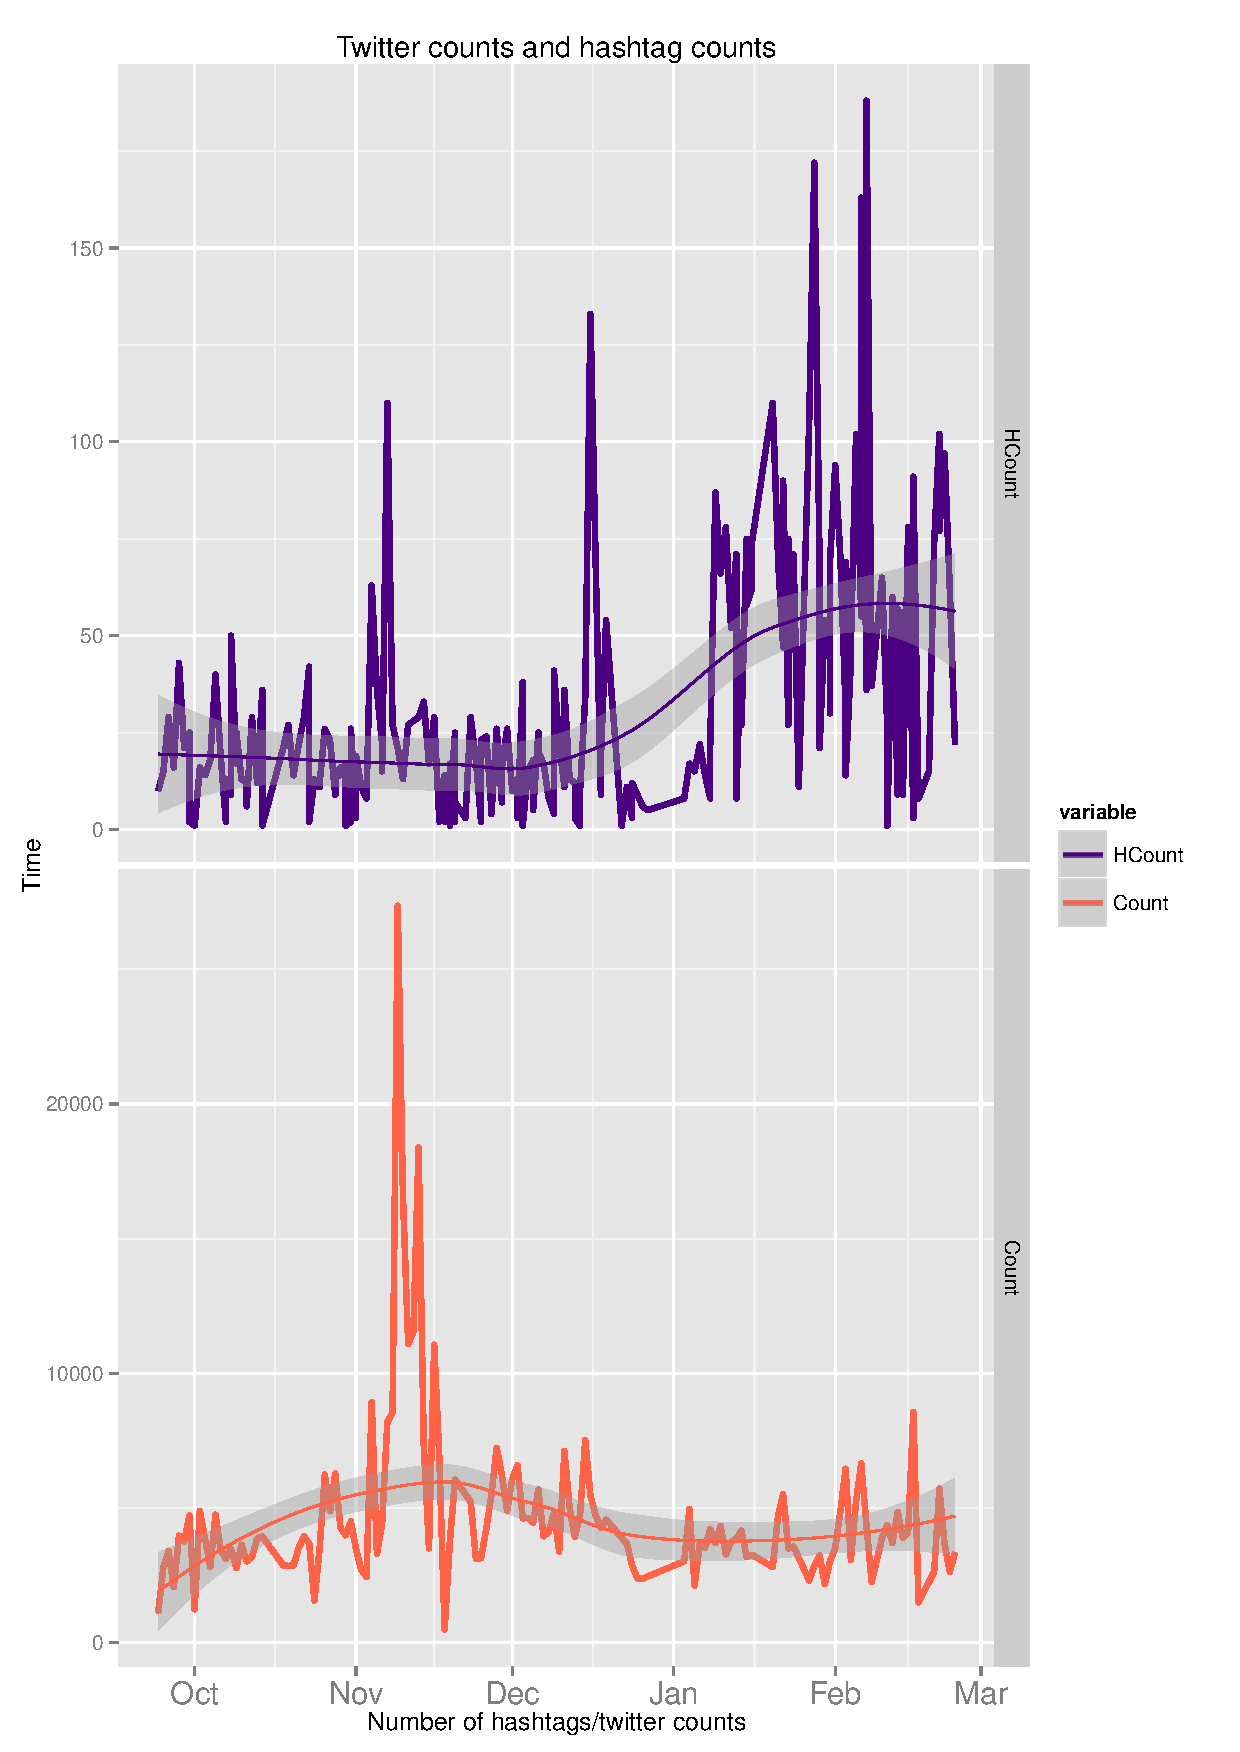
\includegraphics[scale=0.8]{hashtags-vs-counts}
\end{center}
\caption{Hashtags (HCount) and Twitter counts (Count) for London. As we can see both of them have the spike in mid November, but with Hashtags it's quite hard to distinguish signal from noise. The Local Polynomial Regression fit (line) shows the overall trend.}
\label{hashtag-count}
\end{figure}


The main thing that made me consider this option altogether is because the computation cost of finding those hashtags was minimal. Since they are already pre-processed and can be found in a separate attribute I didn't even had to look at the text. The implication of that was that I could easily reduce my dataset significantly, since I'll be throwing away most of the information. All in all the CSVs for every partition of my dataset are about 60 MBs, which is very small compared to the working set of 45 million tweets I had for the occurrences paired travel terms. 


I was getting quite optimistic  in thinking that could be a very simple and easy way to solve my problem and get the time series I needed. To my great disappointment it turned out that the volumes of obtained were quite small and overall the data was very noisy, which would have training a model very hard and predictions from them would've been quite bad. 


In Figure \ref{hashtag-count} you can find a comparison of Hashtag counts and counts. They both have the spike in mid November, but the overall Local Polynomial Regression fit shows that the trends in both are quite different. The hashtags spike in February and the counts in November. That's quite a different behaviour and can result to very inaccurate predictions. Another very big caveat with hashtags is that even if a hashtag is related to a place, it's not guaranteed that the hashtag will have the place name in it. The \#Olympics2014 was a trending topic for a week and is set in Sochi, however with the simple model there is no easy way to take that into account and handle it well.


The fact that they didn't work as my main Twitter feature does not mean I did not use them at all. They are incorporated in the 2nd version of the model (MultiFeatureTwitter) where I am looking at all the words that co occur with a particular place name and using those as additional features. I am going to discuss that in more detail in Chapter \ref{chap:model} on page \pageref{chap:model} describing how that is used and why it could be beneficial to do so. To conclude - hashtags are useful not as a single input, but rather as an additional feature that can be used to enrich the model.



\subsection{Occurrences paired with travel terms} 
\label{sec:tweettext}

The simplest solution I could think of did not work as I had planned. Because of that I had to go back to the drawing board and think of another way to get everything I need from the data. 


The next thing that seemed worth trying was to start using the actual tweet text and do some processing on it in order to get counts for the place time series. In terms of computation that was much more expensive, because even though the tweet text is limited to 140 characters, when you have 650 million tweets it turns into a non-trivial task. 

In order to form the Twitter time series I excluded all the tweets that do not contains a place name and/or one of the travel words. In Figure 4.1 you can find all of the travel-related words which I used in order to perform the filtering. I picked them by trying to thing of all the words that someone would mention when going on holiday in any way -- hence why ``fly'', ``land'' and ``trip'' are all in the dictionary. 


\begin{figure}[]
\begin{center}
\begin{lstlisting}
terms = {
          "airport": "",
          "check-in": "",
          "fly": "",
          "land": "",
          "landing": "",
          "plane": "",
          "take off": "",
          "destination": "",
          "journey": "",
          "passenger": "",
          "route": "",
          "travel": "",
          "travel agent": "",
          "trip": "",
          "charger flight": "",
          "cruise": "",
          "excursion": "",
          "hostel": "",
          "hotel": "",
          "luggage": "",
          "motel": "",
          "package holiday": "",
          "self-catering holiday": "",
          "sightseeing": "",
          "go sightseeing": "",
          "suitcase": "",
          "tour": "",
          "tourism": "",
          "tourist": "",
          "vacation": "",
          "rail": "",
          "go by rail": "",
          "railway": "",
          "railway station": "",
          "road": "",
          "voyage": "",
          "board": "",
          "go on board": "",
	}
\end{lstlisting}
\end{center}
\caption{All the travel related terms I used in a dictionary. They were used as a very primitive additional filter to capture only the most relevant tweets. }
\end{figure}

%
%As a consequence, I had to perform a lot of substring checking -- checking whether any of the words or any of the place names is in the tweet text, keeping counts of all of those, etc. That in itself is fairly hard to optimise and when working on big sets of data even the smallest improvement could mean a reduction of about half a day or even a day in processing time. 


In my initial setup I had a few steps in order to get to the final time series:
\begin{enumerate}
\item Go through all of the data and take only the relevant tweets reducing the full set to a working set (around 10\% of the overall).
\item Traverse the smaller set and generate the Twitter count time series for a destination -- city or country. 
\end{enumerate}

I decided to partition the data into flat files by having approximately one day in every separate file. Initially everything was well, but after doing the processing a few times I realised that there was an error -- every time there was a new data file I had to reprocess everything again. That wasn't obvious at first, because while the dataset was less than 100GB the total working time was about 3-4 hours, however later it became obvious that this is a bottleneck since everything else depended on getting the data in a format that is easy to feed into the model.

In order to mitigate this I had to think of a better, more efficient and more scalable way of performing that step. My first decision was to combine the two steps into one. So instead of filtering first and traversing the dataset, I now traverse the full dataset and obtain the counts as I go through it. The working dataset is kept, because I need it to extract the additional features later. 

Another drawback of the first version was that every time the process stops halfway through I had to re-run it completely, because I did not store any partial counts up to date. Instead, I was storing the full counts and outputting only after I've gone through absolutely every single file. In the second version I am using partial counts for every place and at the end of each iteration of the algorithm those partial counts were merged with the count up to the slice in order to produce the full counts later. That allows me to traverse the data in an easy way and the whole of it is done in about half a day, while with the previous solution it was taking more than 2 days.

\begin{figure}[]
\begin{center}
\begin{lstlisting}
one_word_placenames = obtain_one_word_places()
multiword_placenames = get_multiword()

counts = {}

for file in twitter_data_files:
    for line in file:
        tweet = parse_json(line)
        for word in travelwords: 
            if word in tweet:
                travelWord = True
                break
                            
        for i in multiword_placenames:
             if i in tweet:
                 seen_place = True
                 counts[place][datetime] += 1
                            
        for token in tweet.split(' '): # split the text into words
            if token in one_word_placenames:
                seen_place = True
                counts[place][datetime] += 1

        if seen_place or travelWord:
            writeToFile(tweet)

for place in place_names:
     data = load_file(twitter_counts)
     partial_counts = counts[place]
     data = data.append(partial_counts)
     # group them by the date time and then sum them up
     data.groupby('Datetime')
     data.sum()
     output(data)
    
\end{lstlisting}
\end{center}
\caption{Pseudocode for filtering the data, outputting partial counts and then recombining them into the full time series. }
\end{figure}

You can find the pseudo-Python code in Figure 2.3. For the multiword place names I had to iterate the entire dictionary, because that is the best way. For the single word dictionary I perform lookups against the dictionary that contains them all. I have chosen dictionaries over lists, because amortised dictionary lookups are  \BigO{1}, while list lookups are  \BigO{n}. When you are doing over small lists and dictionaries there is no significant effect on performance, but in our case we are doing it for every line in every file therefore the reduction is much needed.


After the filtering and aggregation of the Twitter time series the working data set is 45 GB of data containing 45 million tweets. The reduced dataset is still much smaller in comparison to the full one. However eliminating the duplication of work made it much easier to re-process the data in a more efficient way and very easy feature extraction later. 


After the processing we have simple time series for a city or country, which are simply the date and the Twitter counts for that date. In Table \ref{twit-ts} you can see how the tabular files containing the Twitter counts look. 

Overall, after doing the processing I have approximately 1500 files containing cities and countries time series extracted from Twitter. Those are then joined with the 2403 CSV files for the searches to those places. After the matching up we have 1377 files for 1376 cities and countries plus one for the overall search and tweet volumes. Each of those files has information on the searches to that place for the day and how many times it was mentioned on Twitter. 

\begin{table}[]
\begin{center}
\begin{tabular}{ l | r }
\textbf{Date} & \textbf{Twitter count}\\
\hline
2013-09-25 &  X \\
2013-09-26 &  Y \\
2013-09-27 &  Z \\
\end{tabular}
\end{center}
\caption{Twitter time series.}
\label{twit-ts}
\end{table}

\section{Exploring the correlation between the time series}

Since now we have both of the time series joined up, it was time to see whether the two time series are correlated. There are several ways which allow one to explore the relationship between two variables. 


The method I chose to do that was the most logical -- carry out the Pearson test between the search volumes and the Twitter counts in order to find out what is the relationship in the two. After carrying out the test for all the destinations the results for some were somewhat disappointing.  In Table \ref{r-values} you will find the top and worst 10 destinations by absolute R value, which allows us to see which ones are correlated and which ones not.


\begin{table}[p!]
\begin{center}
\begin{tabular}{ l | r | r | r}
\textbf{Place} & \textbf{P value} & \textbf{R value} & \textbf{ABS R value}\\
\hline
Sochi & 0.00 & 0.78 & 0.78\\
Manaus & 0.00 & 0.56 & 0.56\\
Salamanca & 0.00 & -0.47 & 0.47\\
Najaf & 0.00 & 0.47 & 0.47\\
North Korea & 0.00 & 0.46 & 0.46\\
Marshall Islands & 0.00 & 0.46 & 0.46\\
Faisalabad & 0.00 & 0.42 & 0.42\\
Fukuoka & 0.00 & 0.42 & 0.42\\
Uruguay & 0.00 & 0.42 & 0.42\\
Ukraine & 0.00 & -0.36 & 0.36 \\
\hline
\hline
Des Moines & 1.00 & 0.00 & 0.00\\
Parma & 1.00 & 0.00 & 0.00\\
Burundi & 1.00 & 0.00 & 0.00\\
Quito & 1.00 & 0.00 & 0.00\\
Vieques & 1.00 & 0.00 & 0.00\\
Algiers & 0.99 & 0.00 & 0.00\\
Lampedusa & 0.99 & 0.00 & 0.00\\
La Coruna & 0.99 & 0.00 & 0.00\\
United Kingdom & 0.99 & 0.00 & 0.00\\
Tamworth & 0.99 & 0.00 & 0.00\\
\end{tabular}
\end{center}
\caption{Top 10 and worst 10 destination by absolute R value. Sochi and North Korea have a strong positive correlation, while Ukraine is very negative. As you can see for the worst 10 see it the P value for all of them is nearly 1, which means that for these place any uncorrelated system could produce very similar results as those. }
\label{r-values}
\end{table}

\begin{figure}[]
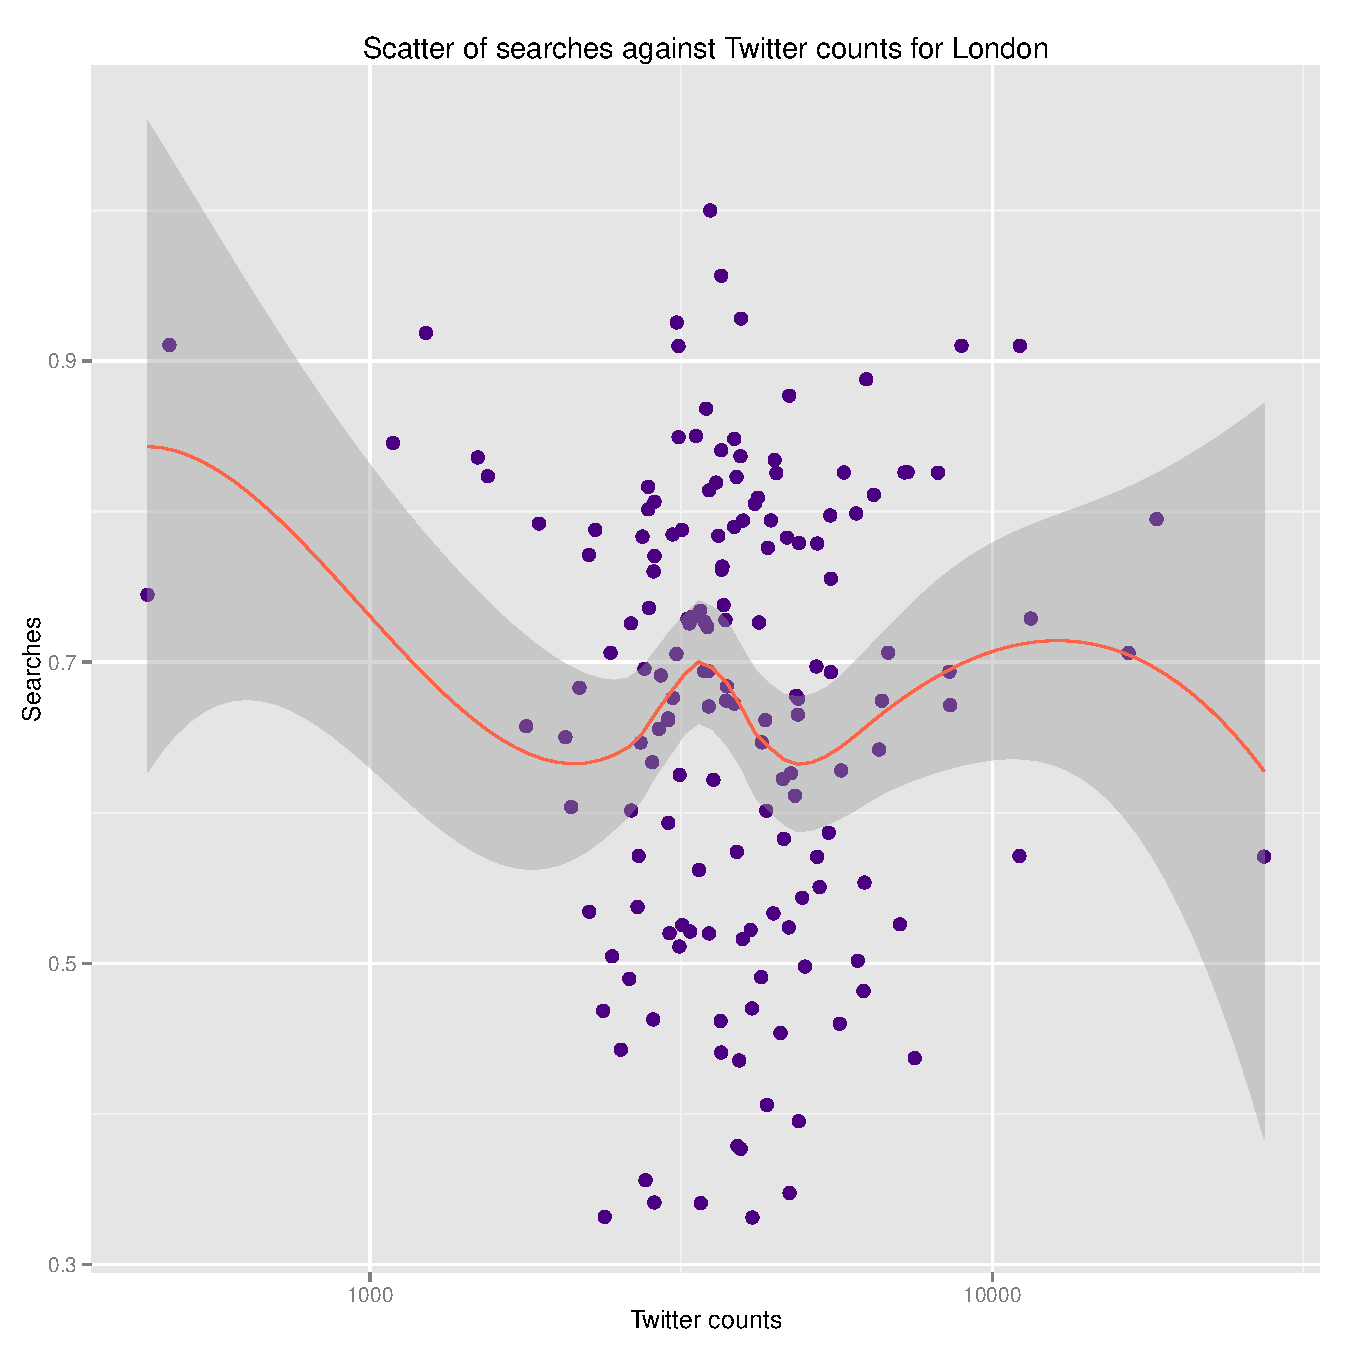
\includegraphics[scale=0.65]{London} 
 \caption{For London the correlation coefficient is 0.003. We can see that there is no clear pattern and the P value implies that two random systems that are not related at all can produce similar result.}
\end{figure}

\begin{figure}[]
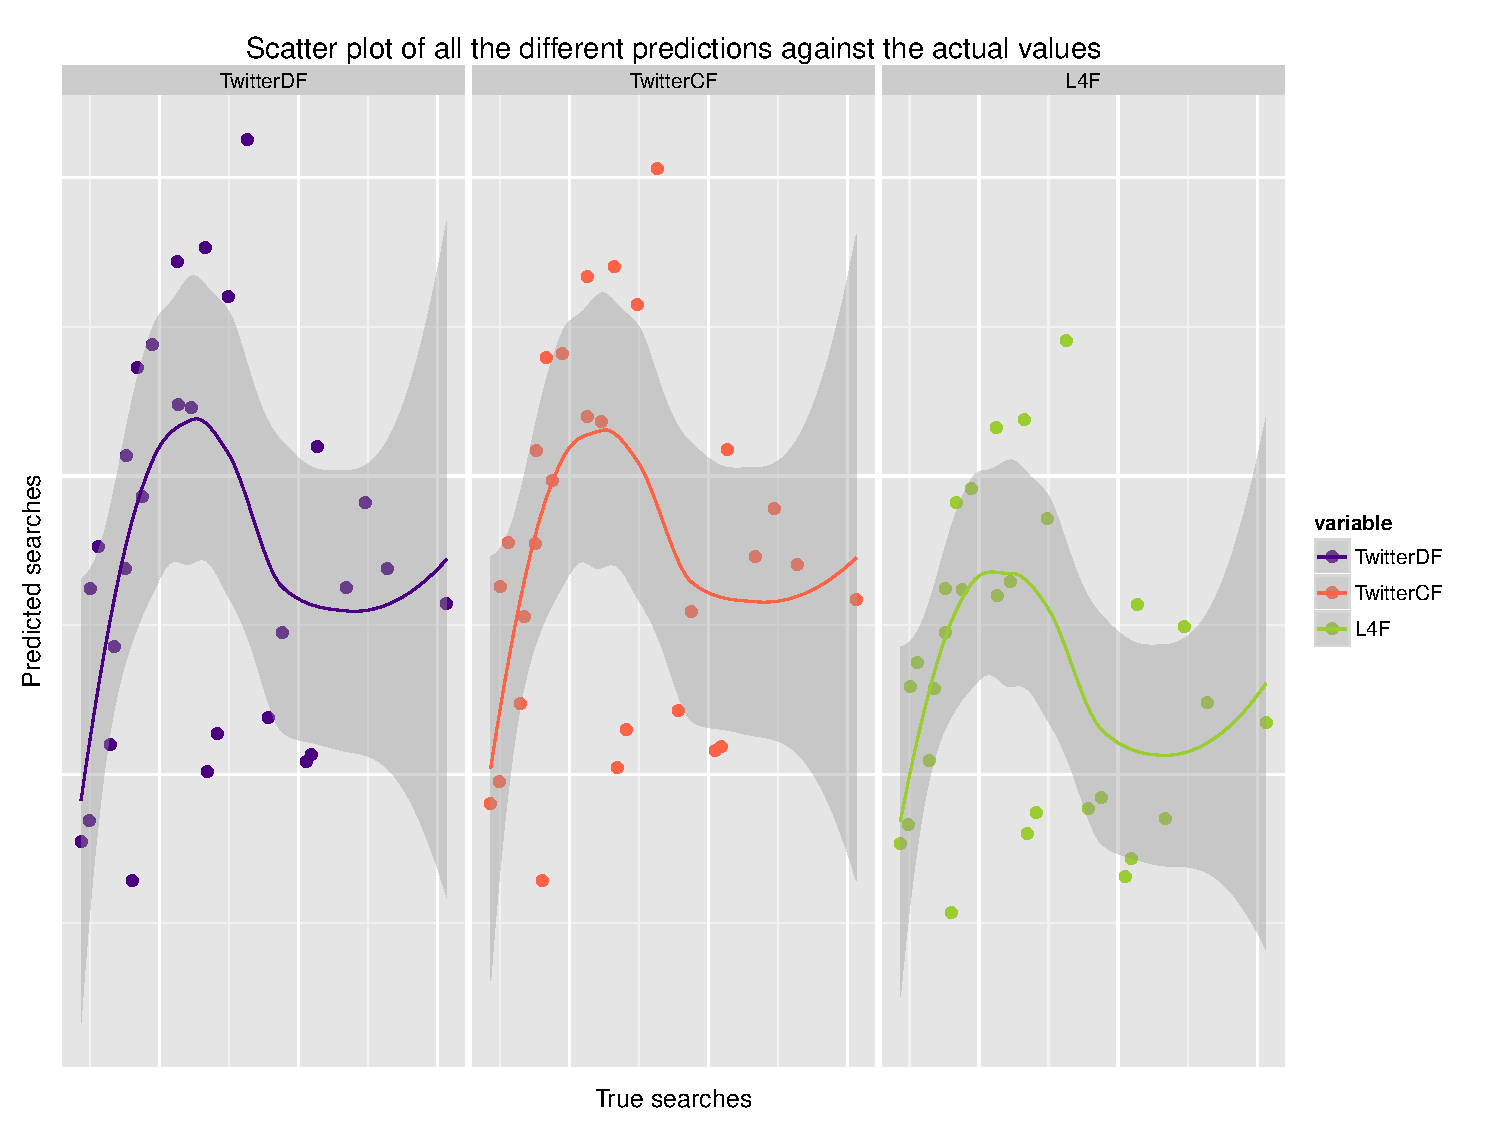
\includegraphics[scale=0.6]{Sochi}
\caption{The Olympiad has bumped the correlation coefficient for Sochi up to 0.77, because people were tweeting and wanted to go and see the Olympiad. }
\end{figure}

\begin{figure}[]
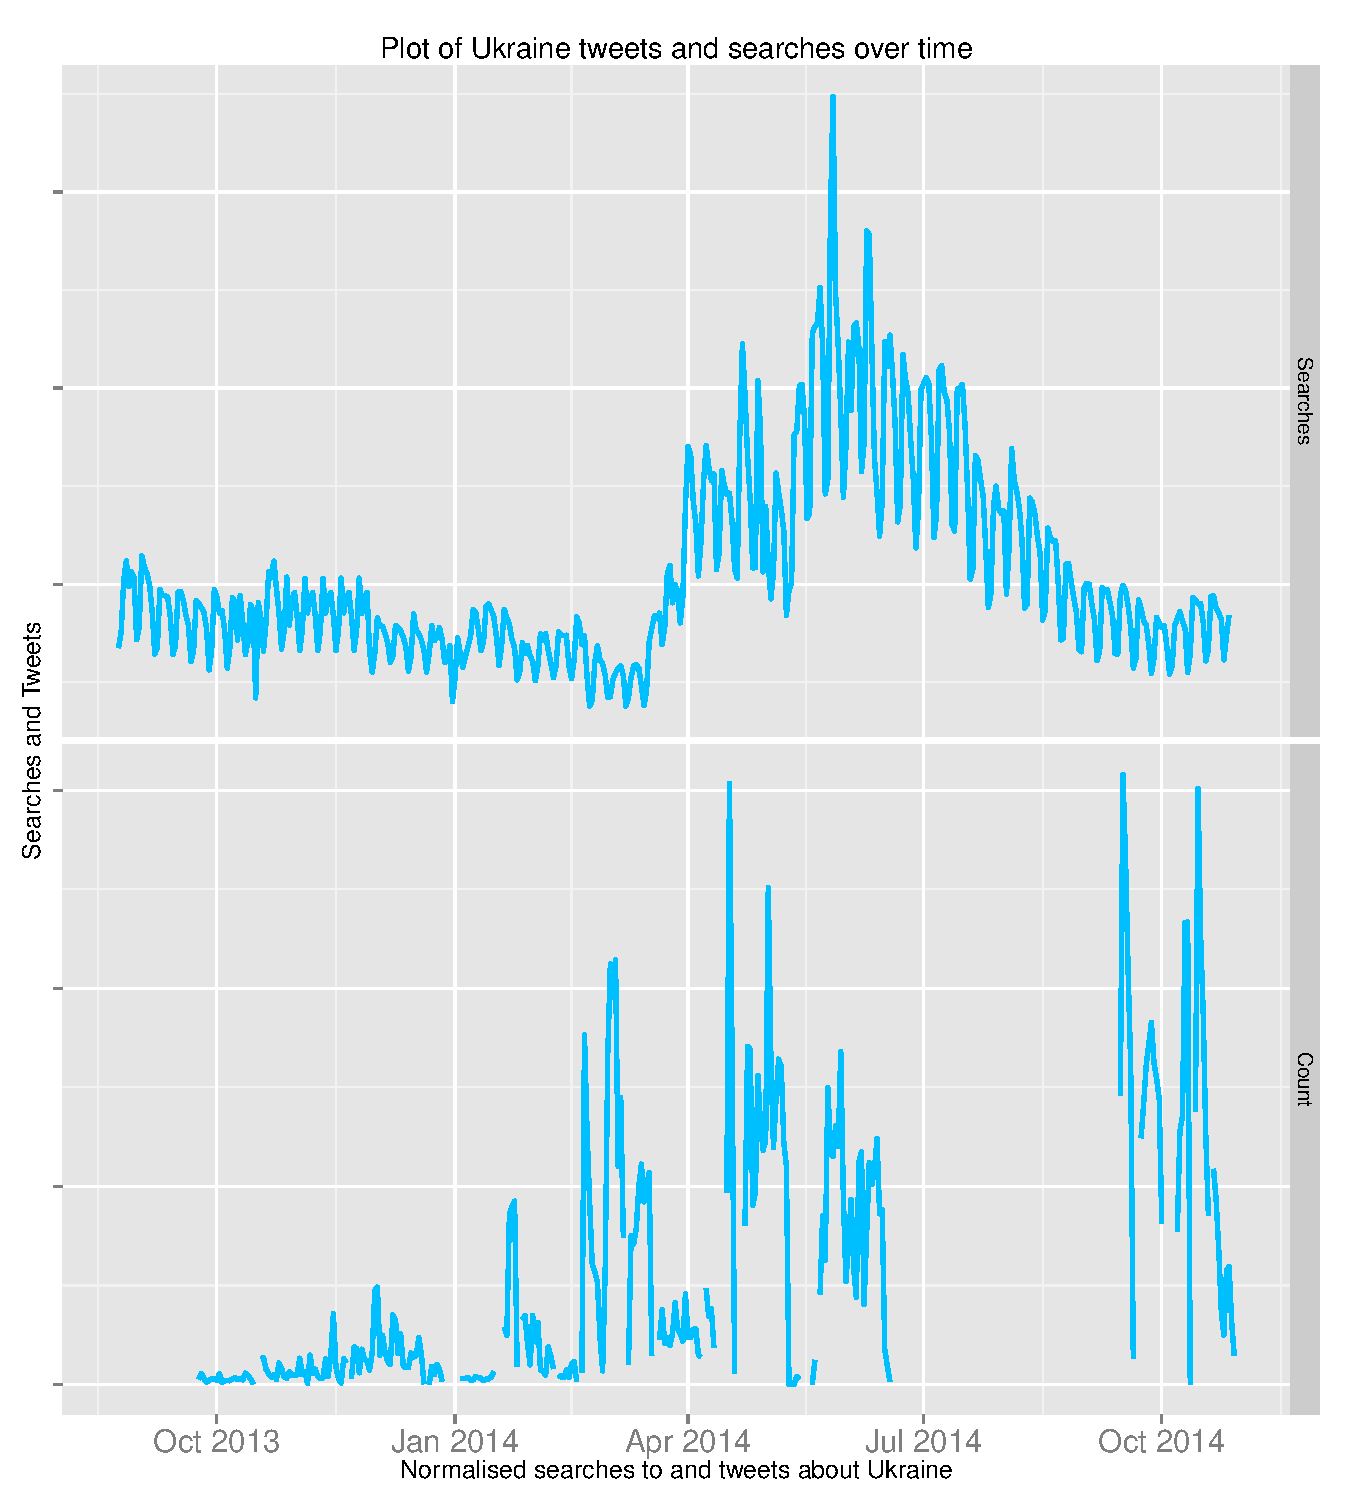
\includegraphics[scale=0.6]{Ukraine}
\caption{Ukraine has a correlation coefficient of -0.35. This is interesting, because the recent protests decreased the number of searches even though people were tweeting a lot, therefore the recent events made them less likely to want to go there. }
\end{figure}

\begin{figure}[]
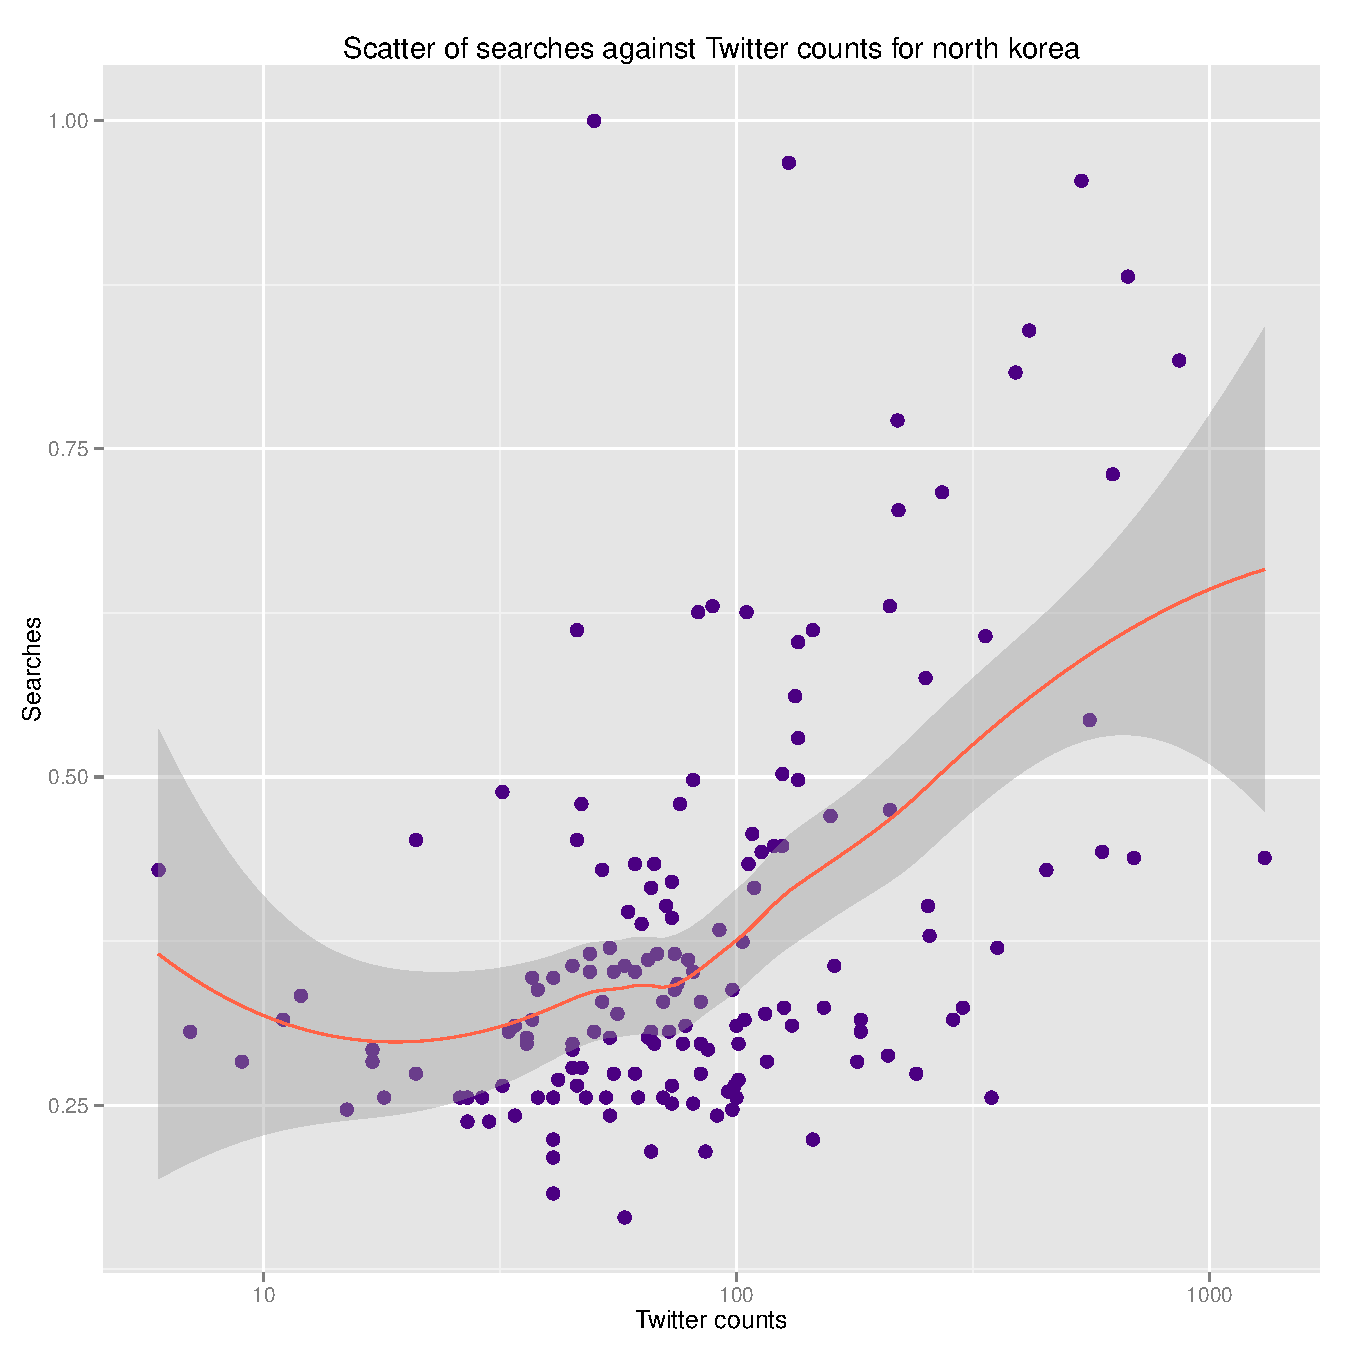
\includegraphics[scale=0.65]{north-korea}
\caption{With a coefficient of 0.45 North Korea is an interesting outlier. Tourism to North Korea is quite a niche market and even though the sentiment is usually negative, people want to go there nonetheless.  }
\end{figure}


All in all, 1286 of the places had an R value of less than 0.2 and the remaining 91 have a value of $>$ 0.2. A correlation of such small magnitude is not even worth reporting, however, since my task it not solely defined by predicting one attribute from another I wanted to include in order to give a perspective on the difficulty of the task. In Figures 2.4 to 2.7 I have shown 4 examples of particularly interesting destinations. 


The best correlation is for Sochi, which has a correlation coefficient of 0.78. For Sochi we can observe at the top right a cluster of dates which have high volumes of tweets, but also a proportionally high number of searches. As we will see in Table \ref{tab:sochi-table} on page \pageref{tab:sochi-table} quite a few of the features picked out by the model were to do with the olympics -- both the positive and the negative aspect. 

Puzzling for most North Korea has got a similar profile, even though the correlation is not as strong. With a correlation of 0.46 it is the 5th best correlation altogether. Tours to North Korea do exist and therefore every time North Korea is mentioned in the news people try to see whether there are flights to that curious place on Earth.

The correlation for Ukraine is very negative and so is for Kiev, both caused because of the recent problems in the country. What is really interesting would be to try to determine what causes the correlation to improve or what makes it worse. I did not have much time to work on that, but using some NLP techniques I believe it is entirely possible to be even more descriptive in what are the exact factors that influence it. 

London on the other hand has a very small correlation coefficient and it is expected that the Twitter models will not perform as good, since the two variable are unrelated and Twitter is not going to play much part in the prediction. 


For those who have a value higher than 0.2 there is definitely some correlation, which could be pushed lower by all the outliers and holes in the data. Fixing that requires some cleansing of those holes in the data. I've described everything that I did for the cleansing in Section \ref{sec:cleansing}.


These results mean that there is a knock-on impact on the models that need to be used in order to perform the prediction. I wouldn't be able to fit a linear regression, because that will give predictions that are very far from accurate. It also means that when doing the model I wouldn't be able to make one that works just with Twitter or the Twitter features. 

A hybrid method would be needed. We need to be using past search data as a component as well. That will ensure that weights of all the features are balanced. That is because the initial idea is to use Twitter as an exogenous factor with some weight. The best model that could do that job is LASSO \cite{lasso}. Due to the very fact that every place is quite different - apart from those with no correlation whatsoever - I fitted a model for each one and one for the overall searches and tweets, which can be found in more detail in Chapter \ref{chap:model} on page \pageref{chap:model}.


\section{Data cleansing}
\label{sec:cleansing}


As I have previously mentioned there are two data sources which I used for this project - data obtained from the Twitter Streaming API and the Skyscanner search volumes. Even with one you can always experience some outages and problems. In this project I used two, therefore there are a couple of sources of risk:
\begin{enumerate}
\item The script that collects data from the Streaming API - sometimes the API just wouldn't work. 
\item The searches data coming from Skyscanner being incorrect or partial - not spanning the full date range.
\end{enumerate}


The dates with incomplete or missing data can impact the regression negatively so it was vital to tidy up all of the data by either backfilling it or filling/removing the missing values. 

As far as the Skyscanner dataset is concerned I have backfilled of data missing by using the Last 4 Fridays, method described in detail in Section \ref{sec:baseline}, in order to ensure that there are enough data point for carrying out all the tests. For the twitter counts, I have simply taken the mean for the values of missing Skyscanner data and dropped all the days where the Twitter collection had problems. For the full features I've just filled the missing values with 0, since there wasn't any better of filling those without removing all the hashtags and words that appear around a specific time and then disappear again.


\section{Feature extraction}
\label{feat-extraction}

With the whole dataset prepared for the statistical analysis and model I wanted to prepare additional data, which was going to enrich the prediction and perhaps make the model a bit more robust, since now it was going to incorporate  more features. With those features one can easily do a better deep dive by re-training the models in order to see which features are the most  helpful in terms of bettering the prediction. I thought that there is also going to be some data on what events were happening during that time, because quite a few of the feature are not going to be present for absolutely day -- the Olympics for instance was trending around the event and significantly improved the correlation for Sochi. 


As an additional note, I am not taking \textit{absolutely} everything that co-occurs. Since humans are fallible and Twitter is a place where everything can be found, I had to remove some weird characters which are used to form the basis of what is called ``ASCII art" and all the different ``emojis'', which are basically emoticons.


This was a computationally intensive task and probably the most difficult bit to get up and running without any major hiccups. What I did for this particular part of the project was something quite similar to what is shown in Figure 2.2, however instead of just adding to the count of a place, I add to the counts of all the words that co-occur with the place name.  Pseudocode of the way it works is shown in Figure 2.8. The algorithm is simple enough, but the fact that the dimensions of the count dictionary are massive I had to be extremely careful not to load up too many of the processed files for extraction at once, because that lead to some memory errors.As a result I decided to split them into partial counts and recombine those. 




\begin{figure}[p]
\begin{center}
\begin{lstlisting}
place_names = get_all_placenames()

counts = {}
# Obtain all the counts
for file in twitter_data_files:
    for line in file:
        tweet = parse_json(line)
  
  	for place in place_names:
	    if place in tweet:
	        # split the text into words
                for token in tweet.split(' '): 
                    if token in one_word_placenames:
                        seen_place = True
                        counts[place][token][datetime] += 1

        if seen_place or travelWord:
            writeToFile(tweet)
            
# Recombination and output the final result

for place in place_names:
     data = load_file(feature_file)
     partial_counts = counts[place]
     data = data.append(partial_counts)
     # group them by the date time and then sum them up
     data.groupby('Datetime')
     data.sum()
     output(data)
    
\end{lstlisting}
\end{center}
\caption{Pseudocode for the feature extraction task.}
\end{figure}


Just in terms of numbers - for London I had 148877 features. The CSV file for London had 148877 (features) times 160 rows (days). It wasn't very easy working with the big sets, because in order to perform all of the predictions they all need to be held into memory, but thanks to Pandas \cite{pandas} the fitting and evaluation of those extended models takes about 2 hours, which is 3 times less than 6 hours without using CSVs and pandas data frames.

\newpage
\section{Tools}


Every one of the aforementioned operations is performed in a separate Python class. The overall system can be separated into several subparts:
\begin{itemize}
\item Collection - scripts/FileStreamer; 
\item Tools for extraction - FeatureExtractor, TwitterExtractor, HashtagExtractor;
\item Processing the data - SearchesProcessor, TwitterProcessor;
\item Tools for the shaping the data - Last4Backfill;
\item Models - Last4Fridays, LassoOverall, ExtendedLasso, LASSOClassifier;
\end{itemize}


I've tried to make the system as robust as possible. All of the classes are as independent as possible of the others to ensure no problems with dependencies. I believe that this could be used as a skeleton to any project that wants to store, process and analyse Twitter data. I am going to put more work next year on creating a well packaged solution for social media analytics that requires minimal input from the user.

The cleaned up version of the code is available on GitHub \cite{code}.






\chapter{Models}
\label{chap:model}


In this chapter we are going to review all of the models that I used in this project to predict the search volumes. I have given the baseline model and the justifications for it. I then go on to describe the models I built - the single Twitter feature TwitterCF and TwitterDF and multi-feature MultiFeatureTwitterCF and MultiFeatureTwitterDF. There is justification provided for the models I have used and also some statistics on them - weight of features and overall improvements. 


\textbf{Note}: I have also trained a RidgeTwitterCF and RidgeTwitterDF. Due to the fact that the results from those did not differ almost at all with the ones produced by the LASSO I have only dedicated a small section at the end of the chapter for them. In the next phase I will train MultiFeatureRidgeTwitterCF and DF in order to see what is the improvement with a bigger feature set.


\section{The baseline model: Last 4 Fridays}
\label{sec:baseline}

The baseline model that Skyscanner has is called Last 4 Fridays (L4F). 
It predicts the daily number of searches and it works in the following way:
\begin{enumerate}
\item We want to predict the number of redirects/searches for this Friday.
\item We take the number of redirects/searches Friday from last week, the week before, etc, until we have the counts form the previous 4 weeks for the corresponding day.
\item We then assign weights to those 4 numbers and assign weights -- the most recent one will get the highest weight, the one after a third and so on.
\end{enumerate}

For any other day of the week it essentially is a tweaked version of an exponential moving average. The formula is $Day=0.675*F1 + 0.225*F2 + 0.075*F3 + 0.025*F4$ where F1 is the same day of the week from last week, F2 -- the week before that and so on.


My colleagues at Skyscanner did some extensive testing on which forecasting mechanism to use in-house for predicting the search volumes. The Last 4 Fridays was tested against a few options like ARIMA, Holt-Winter forecasting, Autoregressive Vector Methods, however it won because of several things:
\begin{itemize}
\item Much simpler to maintain than the other options -- ARIMA has the notion of exogenous factors built-in. It's very tricky to get it right and even if you do, you'd have to tweak them every now and then in order to keep the predictions good. 
\item Because of the weighting scheme you are easily able to capture seasonality, since the most recent day from last week will always have the highest weight.
\item Holt-Winters gave very good forecasts, however the tweaking of $\alpha, \beta$ and $\gamma$ meant that the model might require re-training, which makes it very brittle.
\item The maintenance costs for this one are minimal and the Root Mean Squared Error (RMSE) is comparable to the other models'.
\end{itemize}

A simpler version of this was also considered -- Last Friday. It just assigns different weights to different days of the week. It produces very good results, however in the likely event of an outlier it produces very bad forecasts, so Last 4 Fridays was picked as the overall winner which provides the best trade-off in terms of accuracy and potential for very inaccurate forecasts caused by outliers.

At the end we have a solid forecasting mechanism, which takes into account seasonality and adjusts itself well for any trends. All I had to do is achieve better results with a model that uses social media. 

\section{TwitterDF}
\label{sec:df}

Due to the fact that the correlation between the two time series was either very small or non-existent for the majority of destinations, predicting search volumes solely from Twitter counts was instantly ruled out. That led me to believe that Twitter is meant to be included as an exogenous factor and taking a hybrid approach would be best. For the first iteration I have taken the Twitter counts and the 4 days from previous weeks as features. The model is called TwitterDF where DF stands for Dynamic Fridays, since all the weights are picked on a per city/country basis.

Instead of fixing the Fridays with the exponential scheme used in the baseline I have decided to leave it to LASSO to determine the weights for them. It is very good that we can pick features and also do the regression with a single model. LASSO picks the optimal weights for every feature by minimising its objective function:
\begin{quotation}
\begin{center}
$\underset{w}{min}({\frac{1}{2n_{samples}}} \|Xw - y \|_2^2 + \alpha\|w\|_1) $
\end{center}
\end{quotation}
It is essentially a liner model with l1 reguliser. It solves the minimisation with the least-square penalty for $\alpha\|w\|_1$ where $\alpha$ is the regularisation parameter and and $\|w\|_1$ is the l1 norm of the parameter vector. 

In this particular model there was no great need to tweak the parameter, since we only had 5 features, which we use. But in principal the more you increase $\alpha$ the more the junk weights are penalised hence it prefers sparse solutions with sparse coefficients. 


With this model what we essentially do is take the past search data and include Twitter as an exogenous factor with a different degree of influence, which is the weight picked for it by the lasso. I've trained in total 1377 models - one for every destinations and for the overall volume of tweet counts and searches. All of the weights and raw results can be found in the repository in the directory "results".


\begin{table}[h]
\begin{center}
\begin{tabular}{ l | r | r | r | r | r}
\textbf{Metric} & \textbf{Twitter} & \textbf{F1} & \textbf{F2} & \textbf{F3} & \textbf{F4}\\
\hline
St Deviation & 6.72 & 0.20 & 0.11 & 0.111 & 0.13\\
Median & 0.04 & 0.35 & 0.07 & 0.0082 & -0.01\\
Mean & 0.90 & 0.38 & 0.07 & 0.003 & -0.01\\
\end{tabular}
\end{center}
\caption{Summary of weights for TwitterDF}
\end{table}

The results from this first iteration of the model can be found in Section \ref{TwitterDF} on page \pageref{TwitterDF}. Brief summary -- the overall reduction in RMSE from this model is 4.6\%, which might seem small, but is quite significant, considering the non-existent correlation for some of the destinations.


\section{TwitterCF}
\label{sec:cf}

Building on the improvement from TwitterDF I decided to try something alternative in order to improve the prediction a bit more. In L4F we have an exponential weighting scheme for the weights of the previous days from past weeks. In TwitterDF that is not the case since the weights for all the features are determined by LASSO. In order to make it more consistent and decrease the RMSE even further I decided to mirror the L4F approach in a model which would have 2 features - the sum of the exponentially weighted days from past weeks and the Twitter counts. This new model is called TwitterCF where CF is an abbreviation of Compound Fridays. It is simpler - instead of 5 features, we only have 2, since the past search data is reduced from 4 to 1. LASSO picks the weights only for those features and was expected to reduce the RMSE even further. 


This model has 1377 classifiers trained altogether. In Table 3.2 I've given a summary of the representative statistics on the weights, but that is by no means the single source of truth. 

As we can see the median weight for Twitter is 0.00, but that is pulled down, because of all the destinations that have a negative weight for Twitter -- Ukraine and Venezuela being examples here. It seems that for those cases it is because of the unrest in the country or in others due to a general negative sentiment towards in the news. Fridays have a much higher weight of course, because for most of the models that is the feature that is the most beneficial to the prediction. 

\begin{table}[h]
\begin{center}
\begin{tabular}{ l | r | r }
\textbf{Metric} & \textbf{Twitter} & \textbf{Fridays}\\
\hline
St Deviation & 5.13 & 0.24\\
Median & 0.00 & 0.41\\
Mean & 0.11 & 0.43
\end{tabular}
\end{center}
\caption{Summary of weights for TwitterCF}
\end{table}

As hypothesised, there is indeed an improvement. The overall reduction in RMSE against L4F is 5\% and when we compare Twitter CF to TwitterDF we find that RMSE has been reduced by 0.6\% on average across all the models. The results from TwitterCF are discussed in detail in Chapter \ref{TwitterCF} on \pageref{TwitterCF}. 


\section{MultiFeatureTwitterDF and CF}
\label{sec:multi}

Since the simpler TwitterDF and TwitterCF worked really well, I decided to continue exploring and create a more sophisticated model. In order to do that I used the features which I acquired by performing the data processing described in Chapter \ref{feat-extraction} on page \pageref{feat-extraction}. For the top 80 cities/countries and 2 additional ones -- Ukraine and North Korea -- I took absolutely all of the words that co-occur with those cities/countries and used them as additional feature. That of course mean that for some places I had more than 100 000 features to work with. 


The massive number of features was not a problem at all for LASSO. I've had a set of values of $\alpha$ -- 0.5, 1, 2,5, 10, 20, 50, 125, 250, 500, 1000, 2000, 4000, 8000, 16000, 32000. Since the more you increase the value of the parameter, the more junk weights you throw away, the RMSE proportional to the number of features with nonzero weights. Even though 32000 is a very big value for the parameter, for some destinations with big number of features it's worth going even further beyond that to reduce the weights to less than 10.


Figure 3.1shows the improvement in RMSE with reduction of number of non-zero weights as alpha increases plotted against the values for $\alpha$ for all two MultiFeature models. As you can see there is a very good correlation between the increase in value of alpha and the reduction of the two plotted things. 

\begin{figure}[]
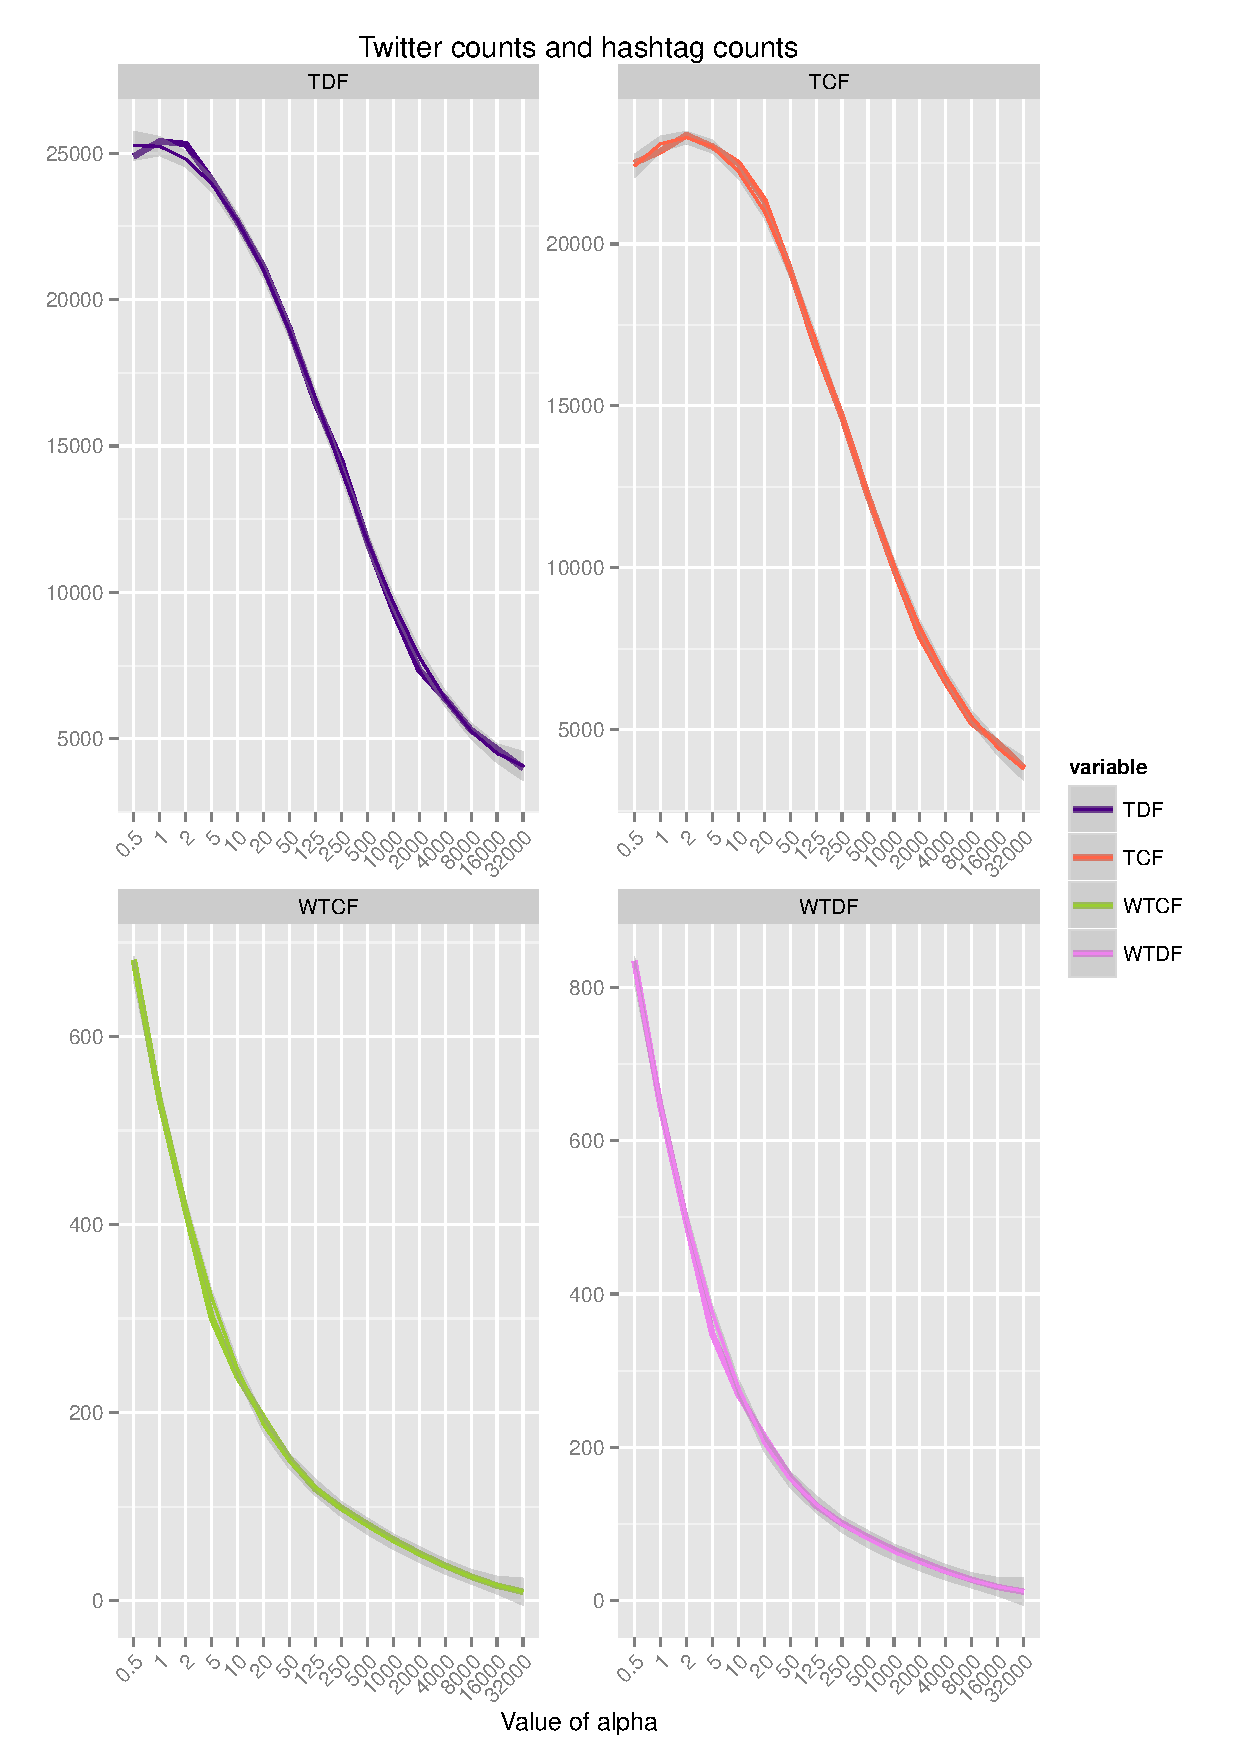
\includegraphics[scale=0.8]{wrmse}
\caption{Reduction of RMSE and non-zero weights as alpha increases. TCF and TDF are the RMSE for MultiFeatureTwitterCF and MultiFeatureTwitterDF respectively. WTCF and WTDF are the number of non-zero weights for the two classifier. The results are means of all the actual values across all models. }
\label{wrmse}
\end{figure}


In Chapter \ref{sec:features} you will find a detailed summary of the results and discussion for the MultiFeatureTwtter models. I have picked several interesting destinations which were the best to show the gains and losses in using the expanded feature set when trying to improve prediction. The model gave mixed results - it improved predictions for some things, but all in all it did not perform better than the simple TwitterCF and TwitterDF.



\section{Model for all the searches}

Since we have got many so many different models for every city and country in the world I also decided to investigate what is the benefit of having one single overarching model. As a result the prediction for the overall search volumes was improved by 3.1\%. The summary of the weights can be found in Table 3.3. It's quite useful having a model for the overall volumes as well because that gives a very quick overview of what is happening. 

\begin{table}[h]
\begin{center}
\begin{tabular}{ l | r | r | r | r }
Twitter & F1 & F2 & F3 & F4 \\
\hline
1.00 & 0.65 & 0.003 & -0.06 & 0.13 \\
\end{tabular}
\end{center}
\caption{Summary of weights for the overall model}
\end{table}


\newpage
\section{Ridge models}

I also trained a few Ridge models that worked on the following basis - taking the weights learned with LASSO, I feed them into the Ridge regression model and classify the data with it. The overall improvement of RidgeTwitterCF and DF over TwitterCF and DF was very small (0.0001\%). Due to time limitations I did not have time to train the RidgeMultiFeatureTwitter models, but I believe that the benefit of using Ridge regression for the classification step will be much greater than the one observed for the single Twitter feature models. 


\chapter{Results}
\label{chap:results}


The lack of any research in this particular area made setting the objectives for this project very difficult. Planning on how to approach and tackle was in itself a challenge as well.. There is no current proposed method of doing this or any measured improvements, so there was no gold standard against which I could benchmark my trained models. In terms of simply benchmarking my models against the baseline I decided to use RMSE as the metric I am striving to decrease.


To get started, I needed to understand the data better and ask myself what I am trying to achieve. As mentioned in the introduction there are two main types of destinations:

\begin{itemize}
\item The ones with constant search volumes to them -- the volumes don't change much over the course of the year -- those are the big cities such as London, New York, Paris and the searches to some countries. 
\item Smaller places such as Ibiza, Alicante, Faro and more exotic destinations such as Lusaka, Tobago and many others that have highly seasonal demand.
\end{itemize}
The difference in the two is graphically represented on the next pages in Figure \ref{london-searches} and \ref{ibiza-searches}. 

\begin{figure}[]
\begin{center}
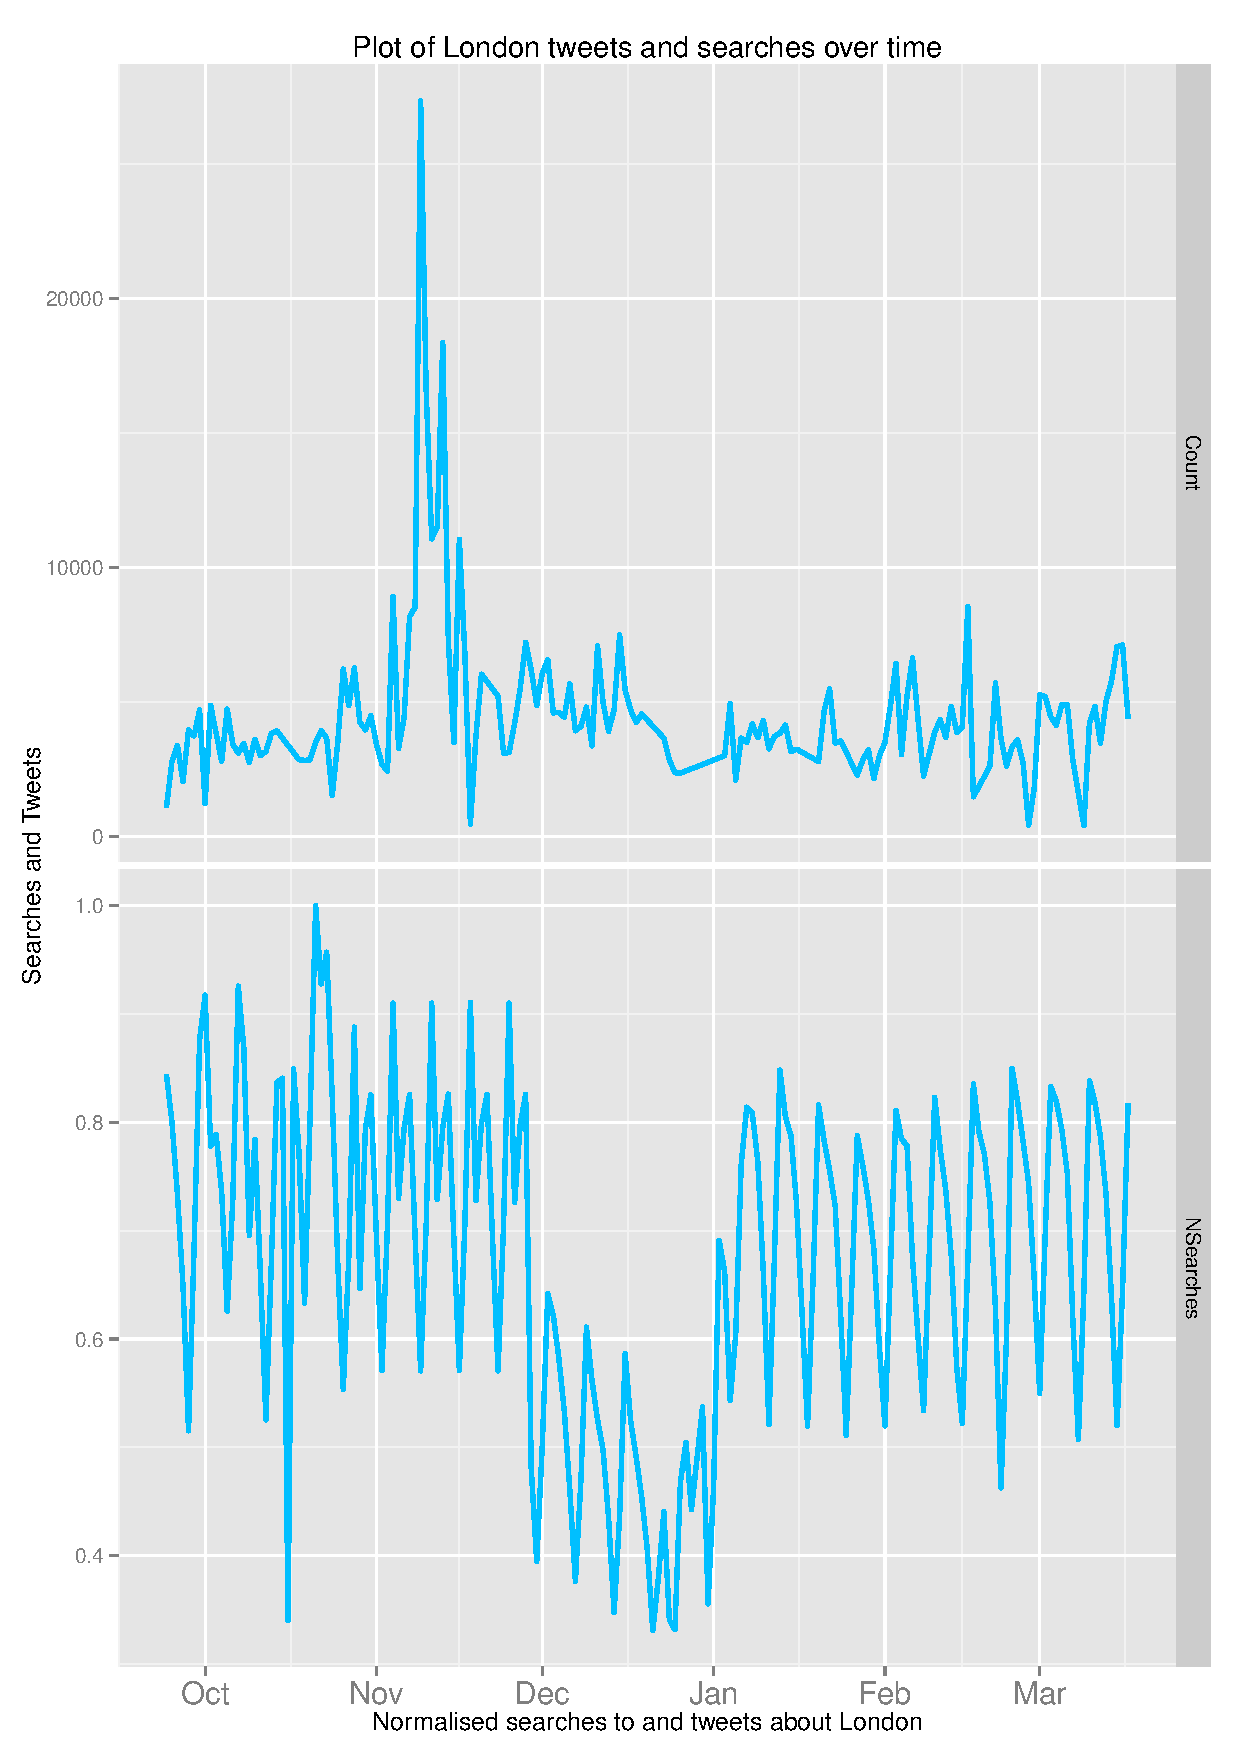
\includegraphics[scale=0.7]{london-searches}
\end{center}
\caption{Searches to and tweets about London - as we can see the trend line  is going to be almost parallel to the X axis.The slight dip in December is due to seasonality. That is noticed across the industry as a whole}
\label{london-searches}
\end{figure}


\begin{figure}[]
\begin{center}
\includegraphics[scale=0.7]{ibiza-searches}
\end{center}
\caption{Searches to and tweets about Ibiza - in this plot we can get the idea of seasonality. The dips is observed as soon as enter autumn and then in January the searches to such destinations pick up again as people are starting to plan their summer holidays}
\label{ibiza-searches}
\end{figure}

Naturally, because of the constant and not so changing nature of the first group, I would expect my model to perform better on the second group. The Root Mean Squared Error from my models on the 2nd group should be smaller or roughly the same as the error generated by the in-house algorithm -- L4F. A more detailed discussion as to why this was picked as the baseline can be found in Chapter \ref{sec:baseline} on page \pageref{sec:baseline}.



\newpage
\section{Results for TwitterDF}
\label{TwitterDF}


Obtaining the initial set of results is vital for any project. In order to get to that stage I had to have working model/s which can perform the task of predicting search volumes with the help of Twitter. As described in Chapter \ref{sec:df}, I picked LASSO for all the feature selection and regressions. 


TwitterDF stands for Dynamic Fridays, which basically means that the weights for the past days are not predetermined as the ones in the L4F exponential weighting scheme, but instead they are automatically picked by LASSO. This way we get an incremental improvement over L4F, but in the model taking into account one of the many exogenous factors that could influence the search volumes either upwards or downwards. I expected that to yield better results for the 2nd group of destinations and possibly for some from group 1.


Overall, I was very pleasantly surprised by the results. On the full set of 1372 destinations which had non-zero RMSE, the first iteration of my model generated better predictions and had lower RMSE on 1034 of the destinations. On the other hand the in-house champion Last 4 Fridays performed better on 338 of the destinations. In order to illustrate that difference there is a scatter plot of the RMSEs in Figure \ref{rmse-scatter}. That means that my model is better on 75.3\% of all the destinations. In the next two runs of training and evaluation, my classifier did better on 74.5\% and 75.6\% of all the destinations. After re-running the experiments, multiple times I am convinced of the significance of the results. 

\begin{figure}[]
\begin{center}
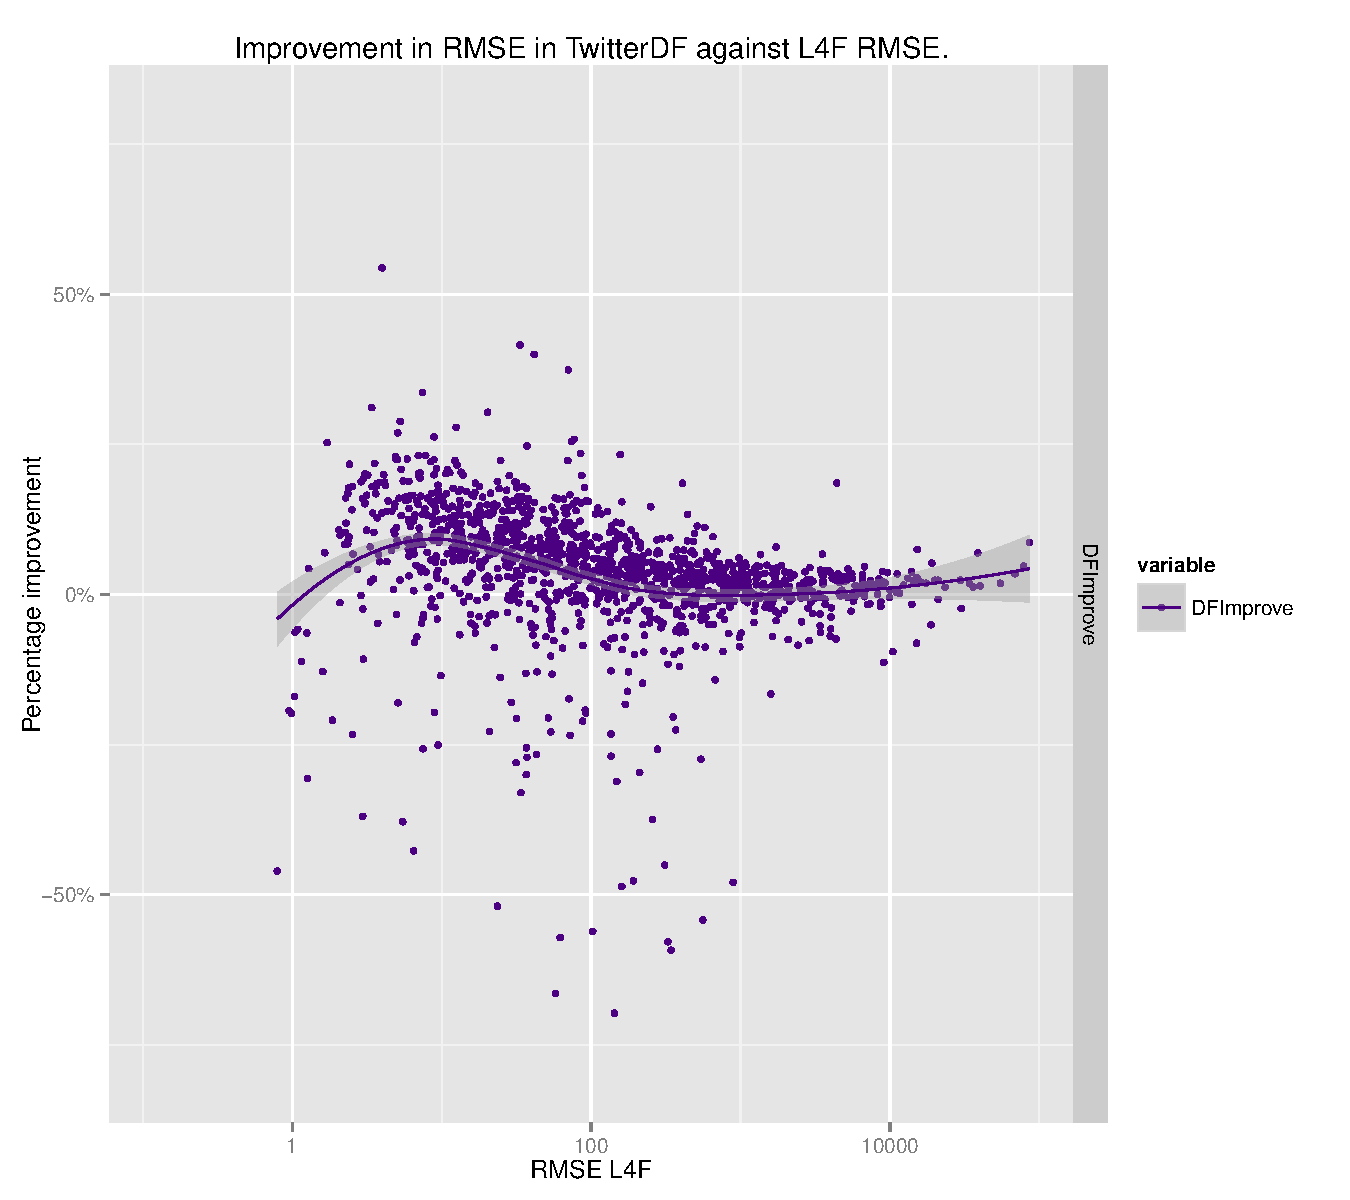
\includegraphics[scale=0.7]{RMSE}
\end{center}
\caption{Scatter plot of the percentage improvement from the TwitterDF model over the baseline L4F. To put things into perspective, I've also plotted the y=x line to make it easier to visualise the border between the two. Anything below the line is where my model performs better and anything above L4F.  }
\label{rmse-scatter}
\end{figure}


In Figure \ref{rmse-scatter} we can see that the performance of the models is actually quite similar. Almost all of the dots are distributed along the x axis. Contrary to my expectations that destinations from group 2 would be better classified by my model, actually it performs just as well on the more constant ones from group 1. 

In Tables \ref{4-1} and \ref{4-2} you can find the places that had the worst performing models and best performing ones in order to give an illustration of what is the improvement and degradation in performance. As we can see in Table \ref{4-1} the destinations here are very small niche destinations, which are very unpopular, so when something happens people are more likely to search to flights to these places. In Table 4.2 we can see something quite similar - overall the decrease for some quite small places with Venezuela being the outlier. Due to the protests the correlation has become very negative and because of that even though people mention it a lot, no one wants to go there, since there is great unrest in the country. 

\begin{table}[]
\begin{center}
\begin{tabular}{ l | r | r | r}
Place & L4F & Twitter & Improvement \\
\hline
Parkersburg & 3.99 & 1.82 & 54.38\% \\
Bismarck & 33.41 & 19.53 & 41.54\% \\
Marshall Islands & 41.63 & 24.99 & 39.98\% \\
Cayo Coco & 70.44 & 44.10 & 37.38\% \\
Yakima & 7.44 & 4.94 & 33.65\% \\
Jonesboro & 3.40 & 2.34 & 31.11\% \\
Casper & 20.30 & 14.14 & 30.34\% \\
Barrow & 5.28 & 3.76 & 28.81\% \\
Niue & 12.50 & 9.02 & 27.82\% \\
Cedar City & 5.08 & 3.71 & 26.91\% \\
Sudbury & 8.89 & 6.56 & 26.24\% \\
\end{tabular}
\end{center}
\caption{Results for destinations that yielded the best improvement in percentage terms when classified with the model from this project in comparison to the in-house one. As we can see they are fairly small niche destinations where it seems that people tweeting about it likely to result in a flight search to that place.}
\label{4-1}
\end{table}

\begin{table}[]
\begin{center}
\begin{tabular}{ l | r | r | r}
Place & L4F & Twitter & Improvement \\
\hline
Hayman Island & 0.12 & 3.06 & -2511.33\% \\
Airlie Beach & 0.65 & 10.17 & -1456.42\% \\
Venezuela & 701.98 & 3277.16 & -366.85\% \\
Crooked Creek & 0.20 & 0.93 & -362.78\% \\
Pereira & 74.94 & 248.77 & -231.97\% \\
Launceston & 122.28 & 404.13 & -230.49\% \\
Jodhpur & 30.80 & 74.05 & -140.40\% \\
Manaus & 295.66 & 707.50 & -139.30\% \\
Del Rio & 5.89 & 13.42 & -127.63\% \\
Trondheim & 257.36 & 573.07 & -122.68\%
\end{tabular}
\end{center}
\caption{Results for destinations that yielded the biggest negative improvement. Quite an interesting mix destinations. The Venezuela result is attributed to Venezuela trending lately, because of the civil uprisings. Eliminating such "negative" influences is one of my goals for next year.}
\label{4-2}
\end{table}


If we look at the top 10 destinations in terms of RMSE (and in flight searches) in Table \ref{top10} we see something quite surprising.  The improvement is positive in 9 out of the 10 examples. Even though it's small, the very fact that there is an improvement, means that taking into account exogenous factors is beneficial and can contribute positively to the quality of the prediction.

\begin{table}[]
\begin{center}
\begin{tabular}{ l | r | r | r}
Place & L4F & TwitterDF & Improvement \\
\hline
Spain & 85,844 & 78,424 & 8.64 \% \\
United States & 78,480 & 74,782 & 4.71\% \\
United Kingdom & 68,706 & 66,335 & 3.45\% \\
Italy & 54,804 & 53,780 & 1.87\% \\
London & 40,129 & 39,554 & 1.43\% \\
Russia & 38,712 & 36,033 & 6.92\% \\
Germany & 36,113 & 35,672 & 1.22\% \\
France & 34,020 & 33,393 & 1.84\% \\
Thailand & 29,997 & 30,701 & -2.34\% \\
Turkey & 29,616 & 28,912 & 2.38\% 
\end{tabular}
\end{center}
\caption{Results for the top destinations by descending RMSE of L4F. 9/10 have lower RMSEs with TwitterDF. As we can see for the top destination - Spain - the improvement is 8.64\%, which is great, because I expected the model to perform worse on places from group 1.}
\label{top10}
\end{table}


\newpage
\section{Results for TwitterCF}
\label{TwitterCF}

As described in Chapter \ref{sec:cf}, the next iteration of the model is called TwitterCF where CF stands for Compound Fridays, because we are taking the sum of the exponentially weighted past days as one single feature. 

The scatter comparison for the two models is in Figure \ref{rmse_scatter_by_reg}. As we can see the improvement of Twitter CF is small, but enough to improve the overall predictions by another 1\%. In order to see how it performs for the different groups of destinations I've plotted the improvement against the normalised standard deviation.

In Figure \ref{rmse-nstdev}, which is just the standard deviation of search volumes divided by the man. That gives us a normalised number which takes into account seasonality - e.g. number who have smaller seasonality are to the left and the ones who are fairly constant are to the right. 

In Table 4.4 I have given the 3 methods and how many times each of them had the lowest RMSE. TwitterCF is the clear winner with 741/1372 places with non-zero RMSE. Overall TwitterCF and TwitterDF have had a smaller RMSE on 83\% of the results, which is a great achievement and proves to show that taking into account other data is beneficial to the quality of the prediction. In the next two re-evaluations the Twitter models achieved 79\% and 84\% respectively. 


\begin{figure}[]
\begin{center}
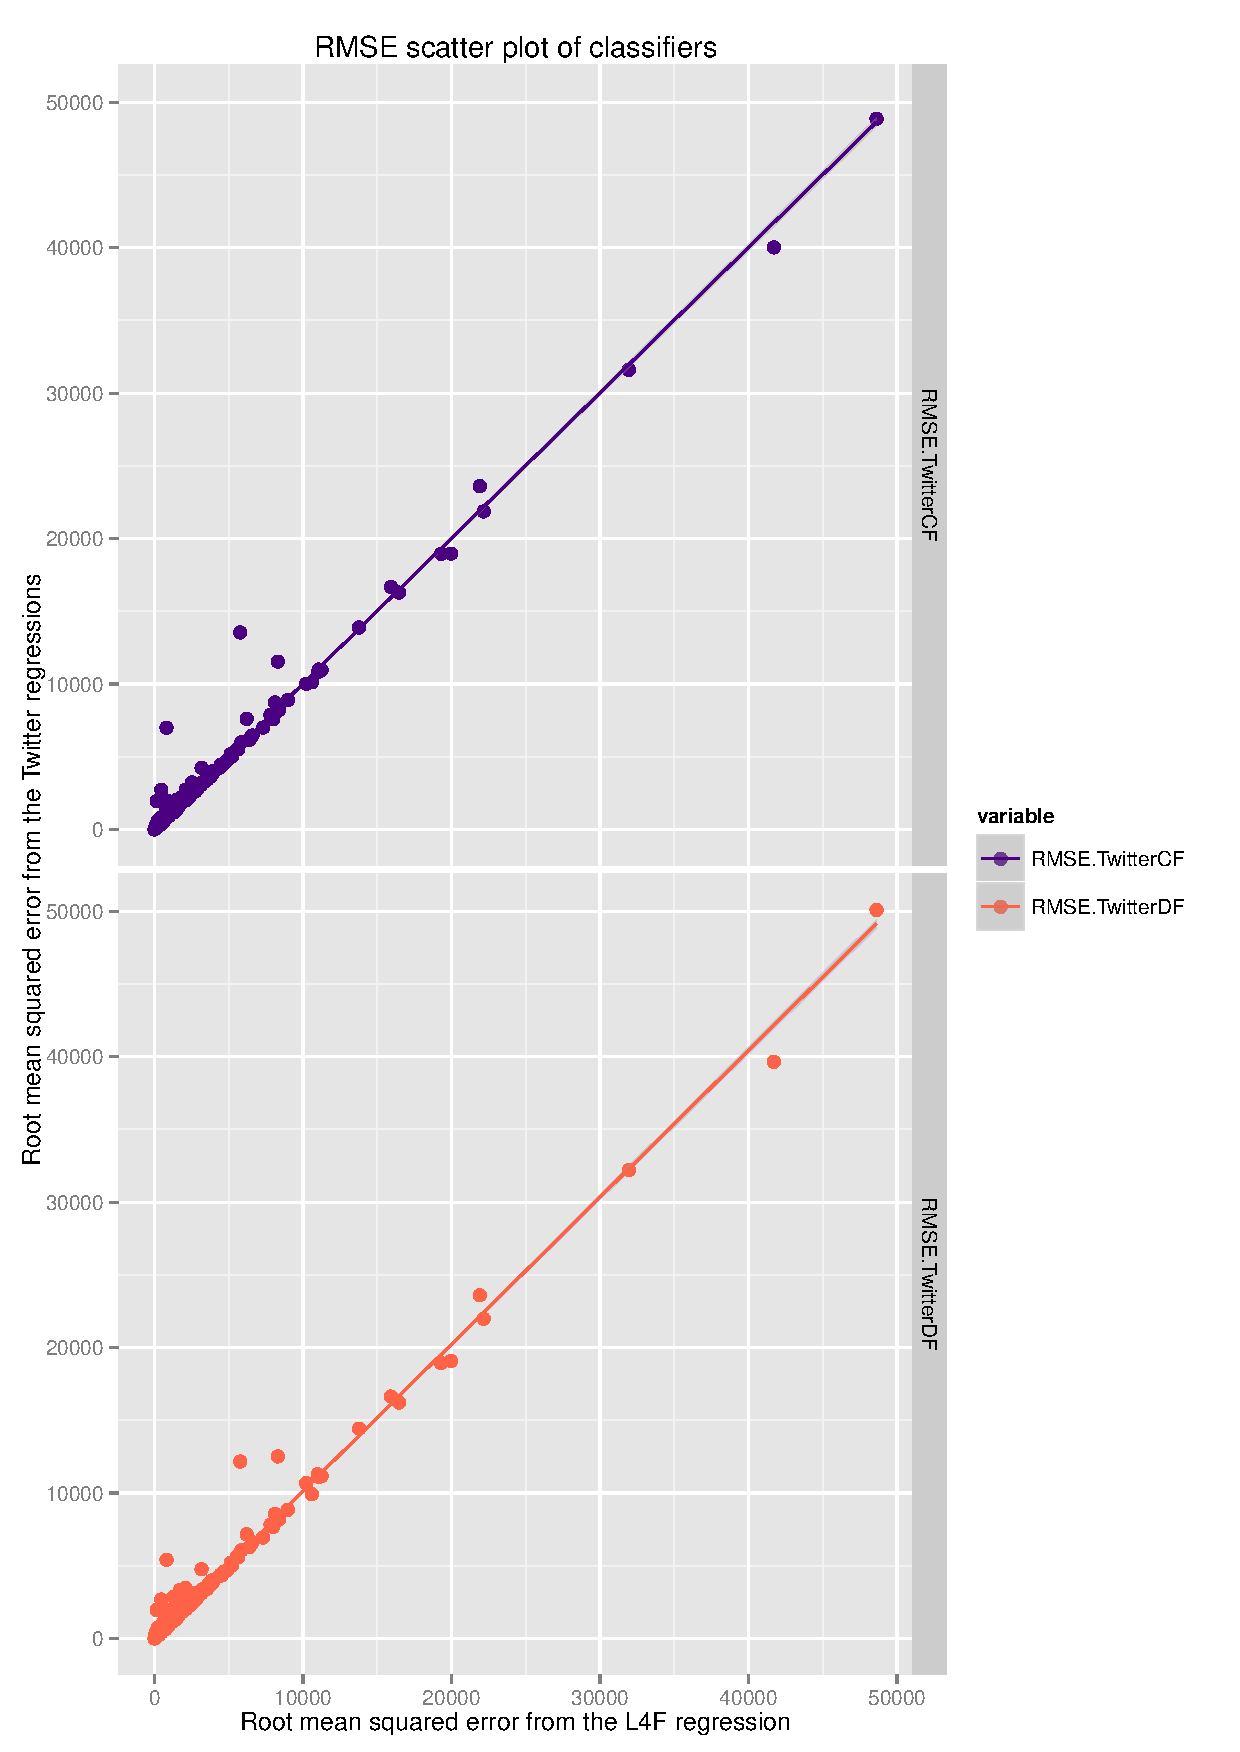
\includegraphics[scale=0.75]{rmse_scatter_by_reg}
\end{center}
\caption{The two models compared: TwitterCF stands for compound Friday -- taking all of the previous Fridays with predetermined weights and using them as a single weight in the regression. TwitterDF is leaving everything to LASSO.}
\label{rmse_scatter_by_reg}
\end{figure}

\begin{figure}[]
\begin{center}
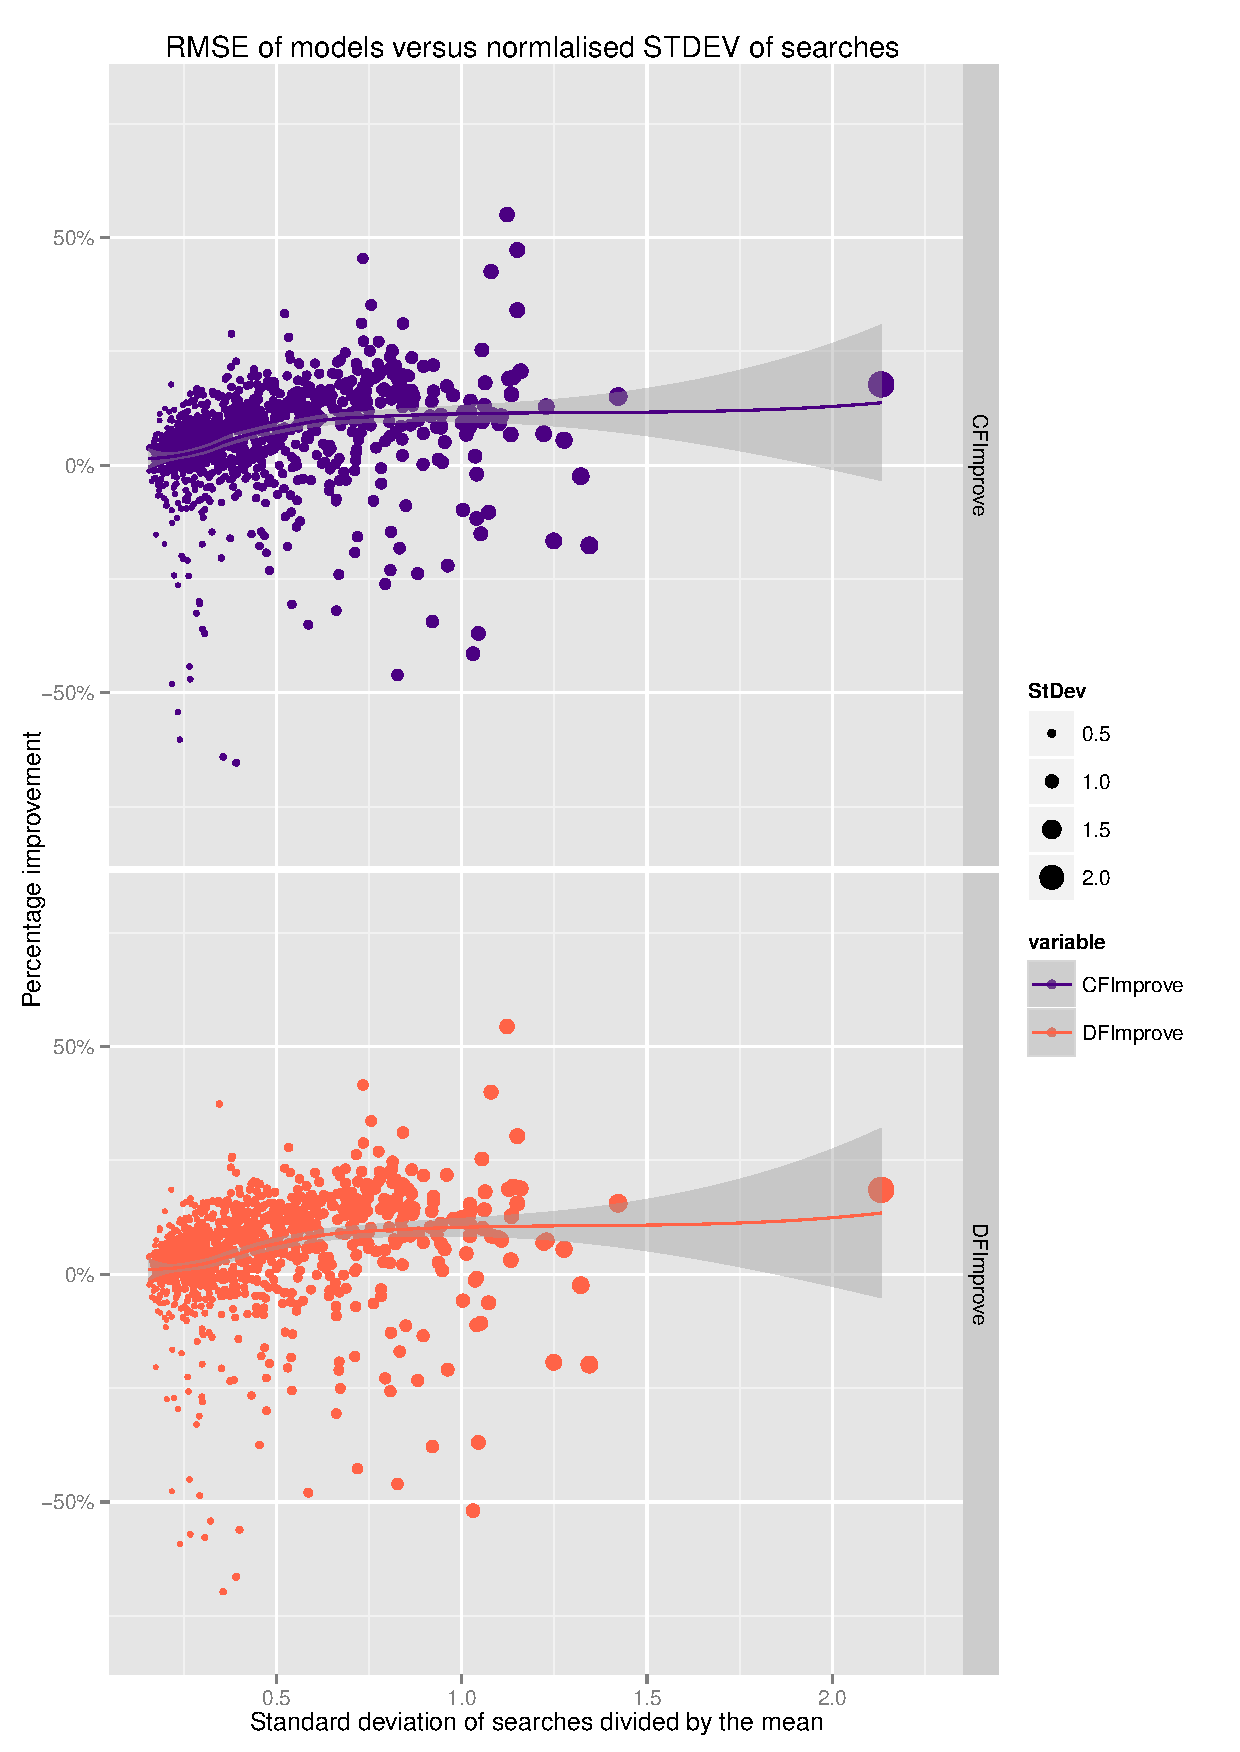
\includegraphics[scale=0.75]{rmse-nstdev}
\end{center}
\caption{Scatter plot of normalised standard deviation (st. dev. divided by the mean) for the number of searches plotted against the percentage improvement for the two classifier over the L4F. On the left is TwitterCF and on the right one can find the improvement for TwitterDF. It seems that the Twitter models are doing good across the whole board.}
\label{rmse-nstdev}
\end{figure}


\begin{table}[h]
\begin{center}
\begin{tabular}{ l | r }
Method & NumBest \\
\hline
L4F & 226 \\
TwitterCF & 741 \\
TwitterDF & 405 \\
\hline
\textbf{Total} & \textbf{1372}
\end{tabular}
\end{center}
\caption{Comparison of the three methods and who had the best results on the dataset of 1372 points. As we can see, the Twitter models have got a definite majority. 83\%+ of the results have the lowest RMSE with the Twitter models}
\label{comparison-all}
\end{table}

In Table \ref{big-table} you can find a more detailed breakdown of the top 20 destinations by RMSE for L4F sorted in a descending order. It includes the improvement of the Twitter models and the improvement of the CF model over the DF one. Overall, the average improvement of the CF model is 0.96\% across all the 1372 individual models for every destination. However the improvement overall ranges from 8.64\% to -3.5\%, which is incredible. That shows again that the TwitterCF model does a very good job in predicting flight search volumes. 


Both of the single feature models did a great job in predicting flight search volumes and now the next step is add more features. 

\begin{table}[p]
\begin{center}
\begin{tabular}{ l | r | r | r | r | r | r }
Place & L4F &  TwitterCF & TwitterDF & Best & Improv. & CF/DF Imp. \\
\hline
Spain & 85,844 & 78,485 & 78,424 & TDF & 8.64\% & -0.08\%\\
US & 78,480 & 73,581 & 74,782 & TCF & 6.24\% & 1.61\%\\
UK & 68,706 & 65,696 & 66,335 & TCF & 4.38\% & 0.96\%\\
Italy & 54,804 & 53,020 & 53,780 & TCF & 3.26\% & 1.41\%\\
London & 40,129 & 39,222 & 39,554 & TCF & 2.26\% & 0.84\%\\
Russia & 38,712 & 36,375 & 36,033 & TDF & 6.92\% & -0.95\%\\
Germany & 36,113 & 35,137 & 35,672 & TCF & 2.70\% & 1.50\%\\
France & 34,020 & 32,816 & 33,393 & TCF & 3.54\% & 1.73\%\\
Thailand & 29,997 & 30,374 & 30,701 & L4F & -1.26\% & 1.07\%\\
Turkey & 29,616 & 28,316 & 28,912 & TCF & 4.39\% & 2.06\%\\
Greece & 23,423 & 22,810 & 23,144 & TCF & 2.62\% & 1.44\%\\
Australia & 21,072 & 20,189 & 20,573 & TCF & 4.19\% & 1.86\%\\
New York & 21,026 & 20,498 & 21,198 & TCF & 2.51\% & 3.30\%\\
Paris & 19,966 & 19,287 & 19,492 & TCF & 3.40\% & 1.05\%\\
Barcelona & 19,087 & 18,237 & 18,093 & TDF & 5.21\% & -0.80\%\\
Bangkok & 18,831 & 19,496 & 19,783 & L4F & -3.53\% & 1.45\%\\
Portugal & 17,429 & 16,694 & 17,103 & TCF & 4.22\% & 2.39\%\\
Netherlands & 16,146 & 15,638 & 15,816 & TCF & 3.14\% & 1.12\%\\
China & 15,212 & 14,188 & 14,074 & TDF & 7.48\% & -0.81\%\\
Istanbul & 15,121 & 14,642 & 14,692 & TCF & 3.16\% & 0.34\%
\end{tabular}
\end{center}
\caption{Comparison of the RMSE generated by the 3 models for the first 20 destinations with highest RMSE for L4F. The Best column indicates who has the lowest RMSE for that destination. Out of the twenty TwitterDF and TwitterCF perform better on 18 of the destinations. The overall numbers can be found in table 2.4. The average improvement of CF over DF is 0.96\%, which even though small is significant nonetheless. }
\label{big-table}
\end{table}


\newpage
\section{MultiFeatureTwitterDF and CF}
\label{sec:features}

As said in the previous section, TwitterCF and TwitterDF performed very well in terms of improving the prediction. The next iteration of the model was called MultiFeatureTwitterDF and MultiFeatureTwitterCF, because I wasn't just using the Twitter counts and the past search volumes for the model. As explained in Chapter \ref{sec:multi} for these two particular models I was taking all the words that co-occur with a place name and use them as features in the predictions. 

In the following subsections I will walk through 3 examples -- Tenerife, Sochi and the United Kingdom. Those are very interesting, because Tenerife is one of those seasonal destinations which are very low-profile during the winter, but after the winter holidays pick up immensely. Sochi is featured because of the Olympic games in February. It is particularly interesting to see how such a big event can influence the searches to a relatively small town in Russia by putting it in the spotlight for 2 weeks. The UK is of course belonging to the group of more steady destinations where there are no significant shifts in demand for flights. 

\subsection{Tenerife}

In Table \ref{table-tenerife}, you can see the results from the MultiFeatureTwitter models on Tenerife. You can see the definite improvement in RMSE for the Twitter models as the number of non-zero weights decreases and the $\alpha$ parameter increases. The other interesting thing is that for $\alpha=1000$ the Twitter classifier become better and the number of weights decreases more and more. In order to illustrate the winning combination of weights I have picked all of the weights in Table 4.7 -- apparently the solar eclipse was very popular and friend is also in the words that add to the prediction. 

In Figure 4.6 I've plotted the actual searches vs the predicted ones. The axis labels are removed for confidentiality reasons. The relationship between the two is quite linear, which means that our predictions is good. 

The conclusion is that MultiFeatureTwitter models are good at predicting the search volumes for destinations that have very well expressed seasonality -- Tenerife, Ibiza, etc. However it's quite vital that the models are re-trained every months or so, because that steps up the seasonality and changes quite a lot of things, especially with the multitude of features on which the model depends on. 

\begin{table}[]
\begin{center}
\begin{tabular}{ l | r | r | r | r | r | r}
$\alpha$ & $>$ 0 W CF & MultiTwitterCF & $>$ 0 W DF & MultiTwitterDF & L4F & Best\\
\hline
0.50 & 191 & 11,683 & 200 & 14,961 & 1,517 & L4F\\
1 & 175 & 12,507 & 177 & 15,647 & 1,517 & L4F\\
2 & 146 & 13,288 & 151 & 15,161 & 1,517 & L4F\\
5 & 136 & 13,607 & 131 & 14,387 & 1,517 & L4F\\
10 & 116 & 12,728 & 114 & 11,341 & 1,517 & L4F\\
20 & 112 & 11,379 & 108 & 8,950 & 1,517 & L4F\\
50 & 88 & 6,601 & 85 & 5,197 & 1,517 & L4F\\
125 & 51 & 1,946 & 56 & 2,009 & 1,517 & L4F\\
250 & 33 & 1,684 & 36 & 1,788 & 1,517 & L4F\\
\hline
500 & 22 & 1,596 & 23 & 1,465 & 1,517 & TDF\\
1,000 & 11 & 1,423 & 13 & 1,593 & 1,517 & TCF\\
2,000 & 5 & 1,356 & 8 & 1,815 & 1,517 & TCF\\
4,000 & 1 & 1,366 & 4 & 1,854 & 1,517 & TCF\\
8,000 & 1 & 1,366 & 4 & 1,853 & 1,517 & TCF\\
16,000 & 1 & 1,366 & 4 & 1,852 & 1,517 & TCF\\
32,000 & 1 & 1,366 & 4 & 1,850 & 1,517 & TCF\\
\end{tabular}
\end{center}
\caption{Improvement in RMSE for Tenerife. As we can see after we get to a certain point the Twitter models get better and better, until it gets to discarding all of the weights, but the Fridays. The optimal result for TwitterCF is with 5 weights and for TwitterDF -- 8, since the reduction in RMSE afterward is negligible, while the DF version performs best with 23 and it starts getting worse. The features and weights at $\alpha = 1000$ are in Table 4.6.}
\label{table-tenerife}
\end{table}


\begin{table}[]
\begin{center}
\begin{tabular}{l | r}
Feature & Weight \\
\hline
time & 583.35 \\
\#tenerife & -87.43 \\
\#solareclipse & 35.74\\
tenerife & -19.29\\
friend & 64.81\\
Fridays & 0.75\\
begins & -30.50\\
heres & 7.72\\
would & -273.96\\
canary & -7.56\\
view & -10.86 \\
\end{tabular}
\end{center}
\caption{Weights for Tenerife at $\alpha=1000$. These are the weights that the TwitterCF model has picked.}
\end{table}




\begin{figure}[]
\begin{center}
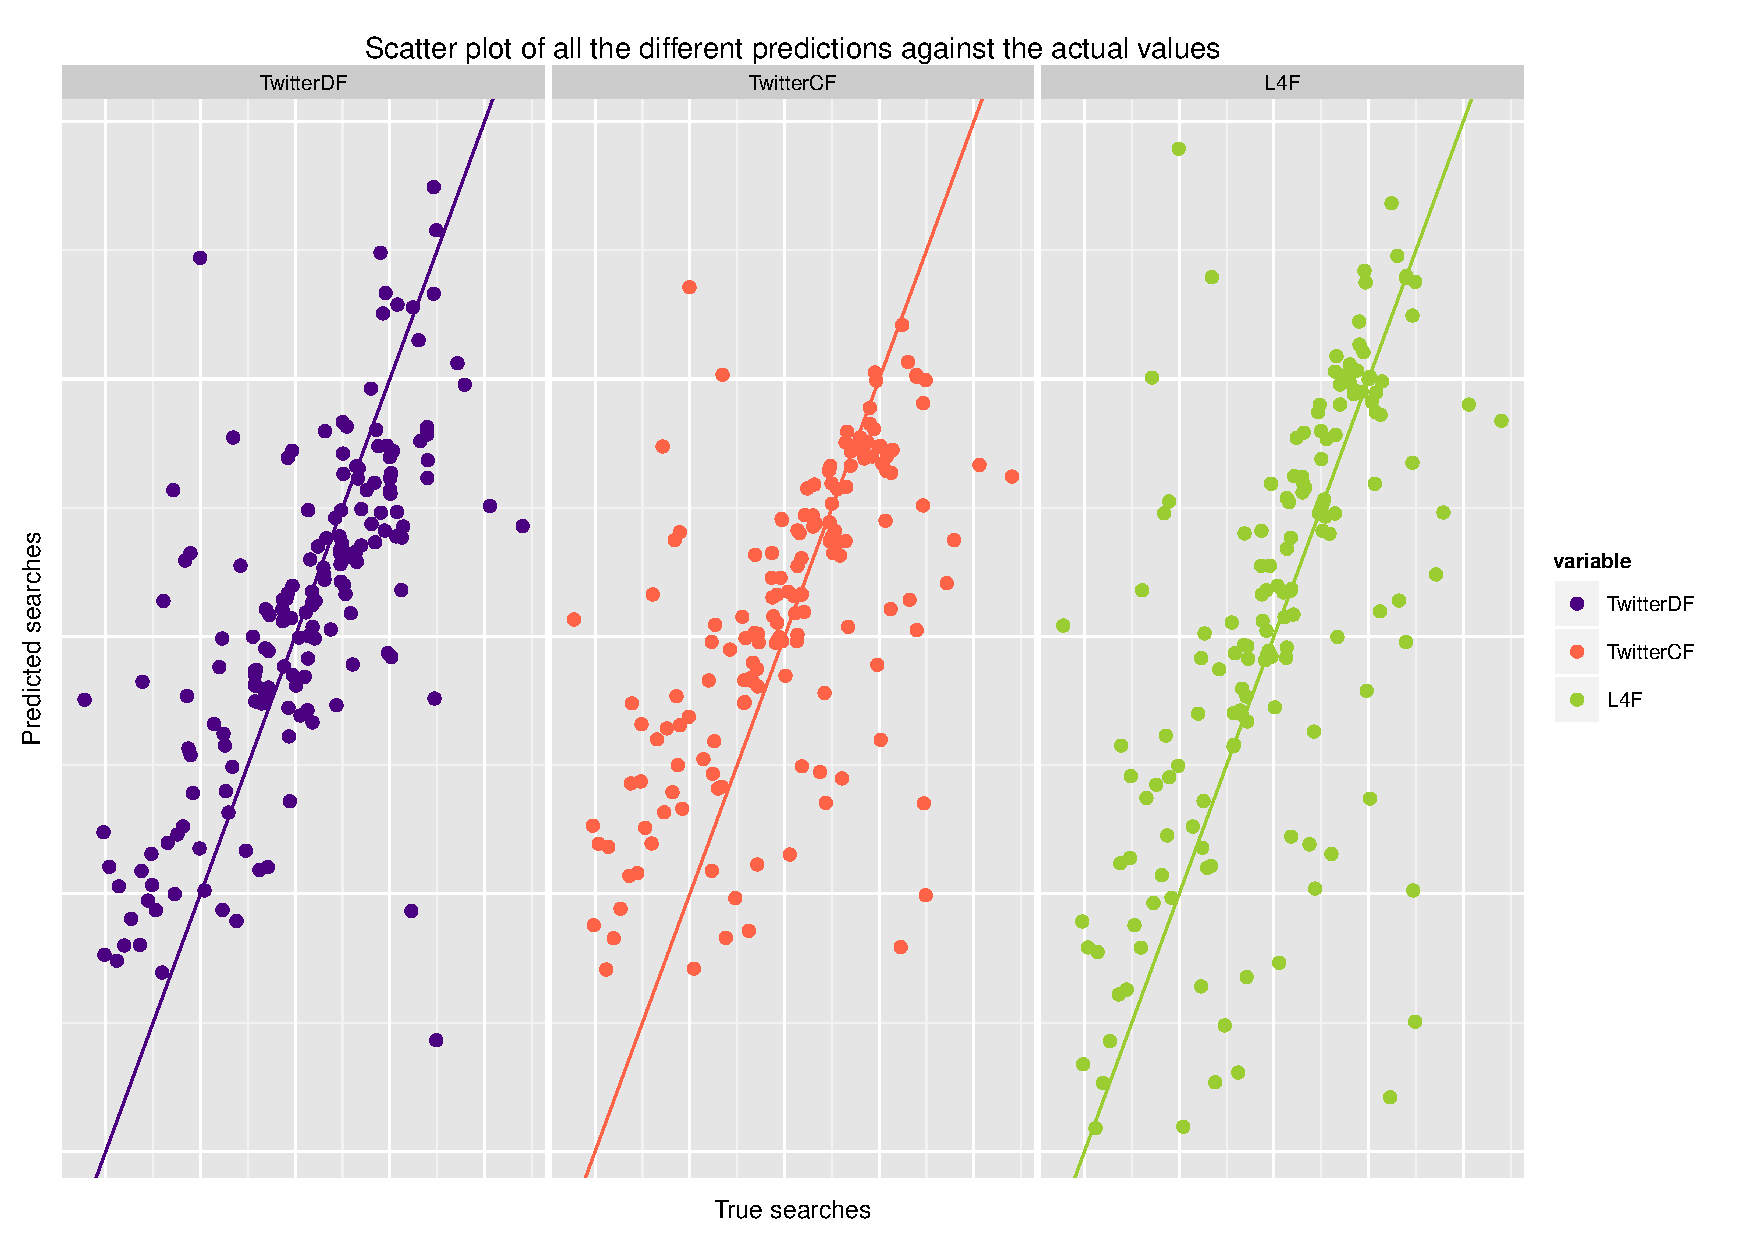
\includegraphics[scale=0.5]{plots/Tenerife}
\end{center}
\caption{Predictions vs actual for a destination from group 2 - Tenerife. For this group Twitter models make actual gains, albeit small. The line $y = x$ is shown to portray the quality of the prediction.}
\end{figure}



\newpage
\subsection{Sochi}


Sochi was picked because of the olympics, of course. The winter event has massively affected the number of searches to Sochi and the number of tweets about it. Just to show the dramatic increase in search volumes, in Figure \ref{sochi-c-s} I have plotted the search volumes to Sochi and tweet counts about it. The increase in searches is roughly 10 times around the Olympics and the number of tweets has gone up from 800/day before to 12000 at the time of the ceremony, which is an increase of 15 times. 

Another interesting side effect of the winter event is that it totally skewed the predictions. In Figure 4.8 I have plotted the predictions agains the actual search volumes -- axis labels omitted for confidentiality reasons again. As we can see there is no clear trend and the points are all over the place. Overall the Olympics made patterns in the data very hard to spot. 


In Table \ref{table-sochi} you can see the RMSE for the MultiFeatureTwitter models for Sochi. The horizontal lines denote the area where the Twitter Models perform better. As we can see it seems that there is a local minima where the MultiTwitterFeature models are better, but then as we discard more and more features, L4F wins at the end. 


The weights for the TwitterDF at $\alpha=500$ are shown in Table \ref{tab:sochi-table}. Again, Olympics dominates the overall picture, with the past Fridays being very prominent features. Interestingly enough, the hashtag \textit{\#olympics} has a negative weight, while \textit{\#olympics2014} is positive. In the next phase of th project I will try to apply more Natural Language Understanding (NLU) in order to find out why are some places more likely to be interesting to people and why. 

\begin{table}[]
\begin{center}
\begin{tabular}{ l | r | r | r | r | r | r}
$\alpha$ & $>$ 0 W CF & MultiTwitterCF & $>$ 0 W DF & MultiTwitterDF & L4F & Best\\
\hline
0.5 & 268 & 10,545 & 377 & 15,909 & 9,156 & L4F\\
1 & 200 & 10,505 & 260 & 15,108 & 9,156 & L4F\\
2 & 170 & 9,976 & 192 & 13,693 & 9,156 & L4F\\
\hline
5 & 138 & 8,774 & 158 & 10,720 & 9,156 & TCF\\
10 & 126 & 8,964 & 132 & 9,808 & 9,156 & TCF\\
20 & 112 & 9,051 & 115 & 10,802 & 9,156 & TCF\\
50 & 99 & 8,867 & 101 & 9,577 & 9,156 & TCF\\
125 & 81 & 9,129 & 82 & 8,604 & 9,156 & TDF\\
250 & 60 & 8,924 & 57 & 8,304 & 9,156 & TDF\\
500 & 41 & 8,335 & 44 & 7,982 & 9,156 & TDF\\
1,000 & 29 & 8,443 & 28 & 8,164 & 9,156 & TDF\\
2,000 & 16 & 8,424 & 19 & 8,341 & 9,156 & TDF\\
4,000 & 7 & 9,143 & 9 & 9,307 & 9,156 & TCF\\
\hline
8,000 & 3 & 9,759 & 6 & 9,938 & 9,156 & L4F\\
16,000 & 2 & 9,727 & 5 & 9,860 & 9,156 & L4F\\
32,000 & 2 & 9,950 & 4 & 10,010 & 9,156 & L4F\\
\end{tabular}
\end{center}
\caption{Improvement in RMSE with the expanded feature set for Sochi, which is in 2nd group of destinations.  
As you can see in terms of absolute value, the RMSE for the Twitter model with compound fridays -- RMSE TCF -- has decreased 20\% for the area where TCF has the lowest RMSE. I have separated the area where the Twitter Models are better with two horizontal lines. The RMSE for TDF is 2 times lower at $\alpha=500$ and that's where the model performs the best. Both models have a comparable number of weights, which is really interesting.}
\label{table-sochi}
\end{table}



\begin{figure}[]
\begin{center}
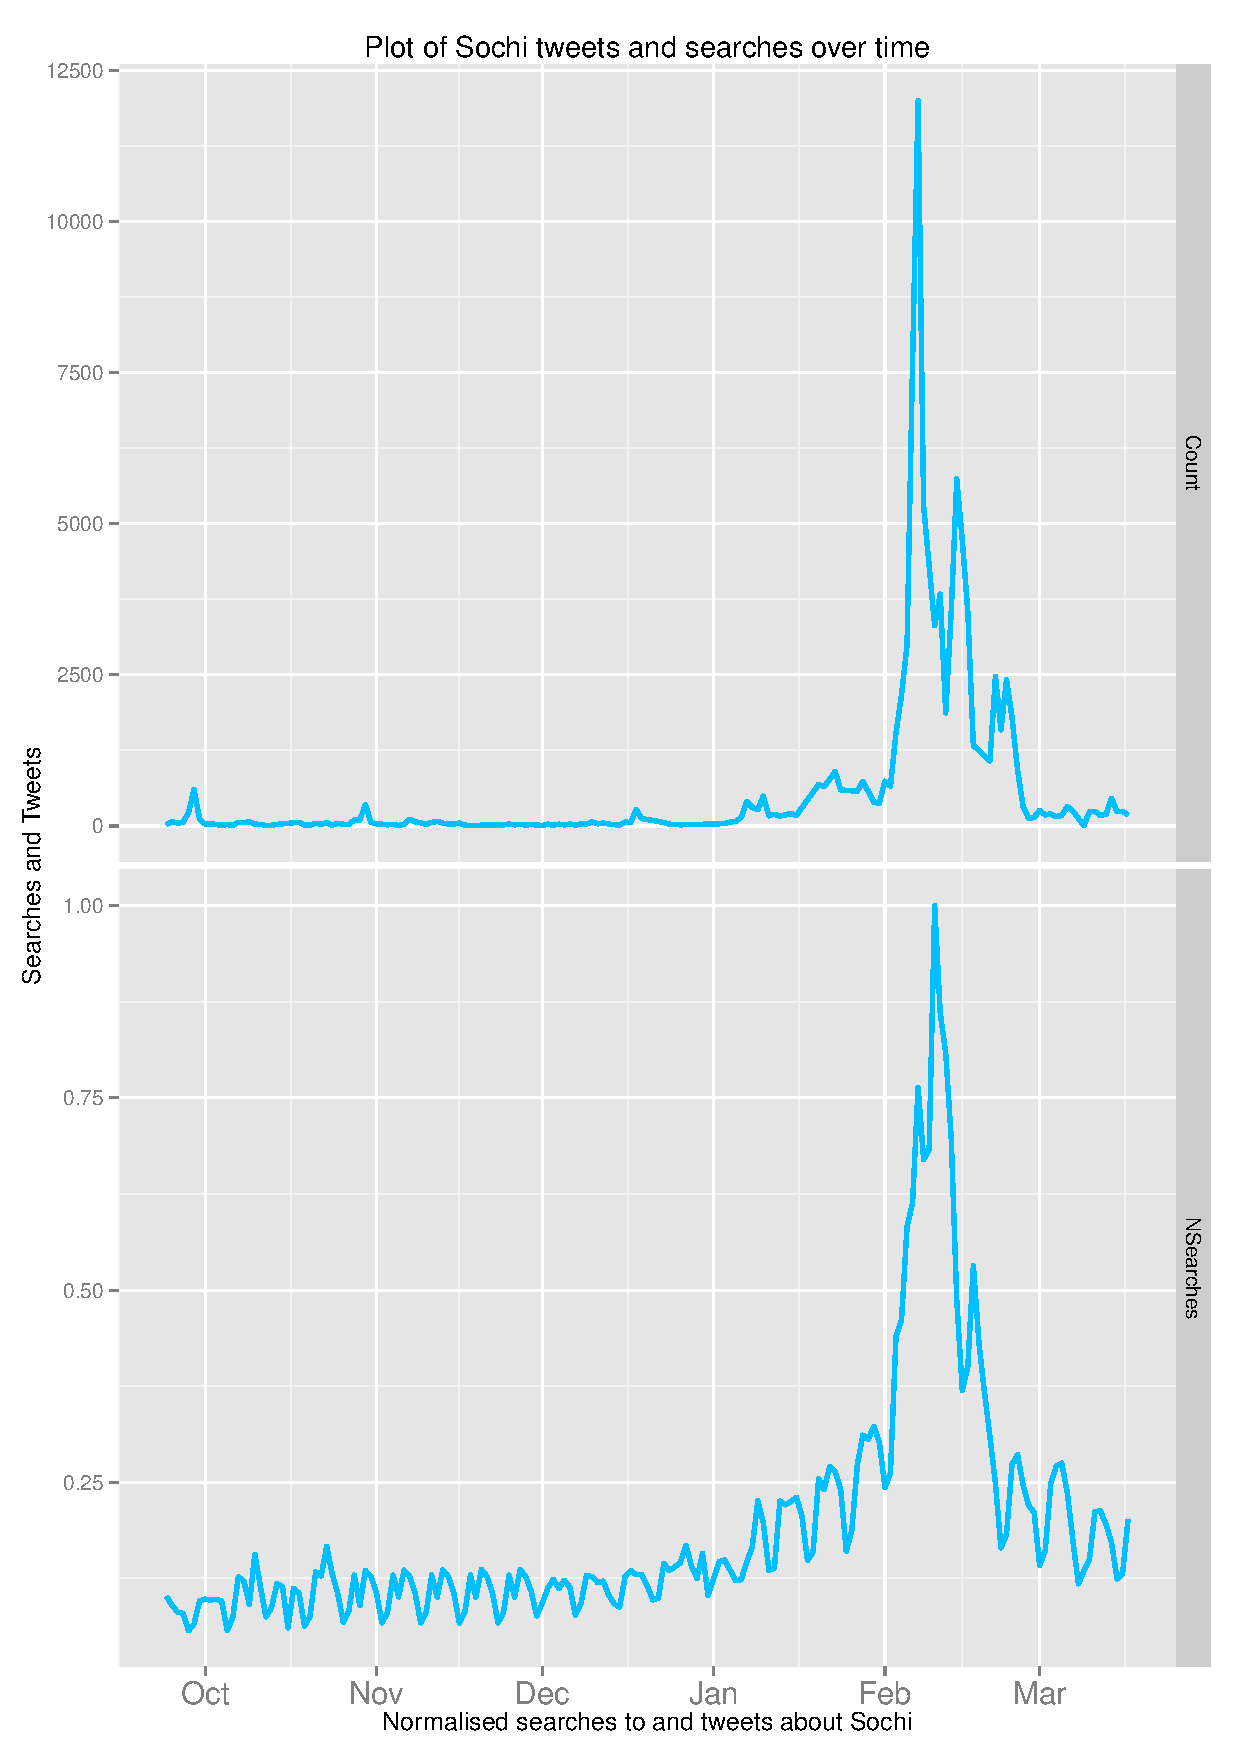
\includegraphics[scale=0.75]{Sochi-s-c}
\end{center}
\caption{Searches and tweets Sochi. The massive spike is the Olympics. As we can see the two time series are correlated and the spike it tweets is just a bit before the spike in searches.}
\label{sochi-c-s}
\end{figure}




\begin{table}[]
\begin{center}
\begin{tabular}{l | r}
Feature & Weight\\
\hline
team & 16.08\\
\#olympics2014 & 2.40\\
Count & 1.34\\
olympic & 1.30\\
Friday1 & 0.75\\
canada & 0.72\\
Friday3 & 0.16\\
Friday2 & 0.11\\
Friday4 & -0.15\\
hotel & -1.07\\
\#seeyouinsochi & -1.22\\
jump & -1.49\\
\#olympics & -2.24\\
dog & -2.56\\
sochi & -2.52\\
\end{tabular}
\end{center}
\caption{Handpicked features for Sochi at $\alpha=500$. The total number of features is 44 and they are the ones picked by TwitterDF. Interestingly enough dog, sochi and hotel very negative weights. On the other hand there are a few positive weights that relate to the olympics.} 
\label{tab:sochi-table}
\end{table}



\begin{figure}[]
\begin{center}
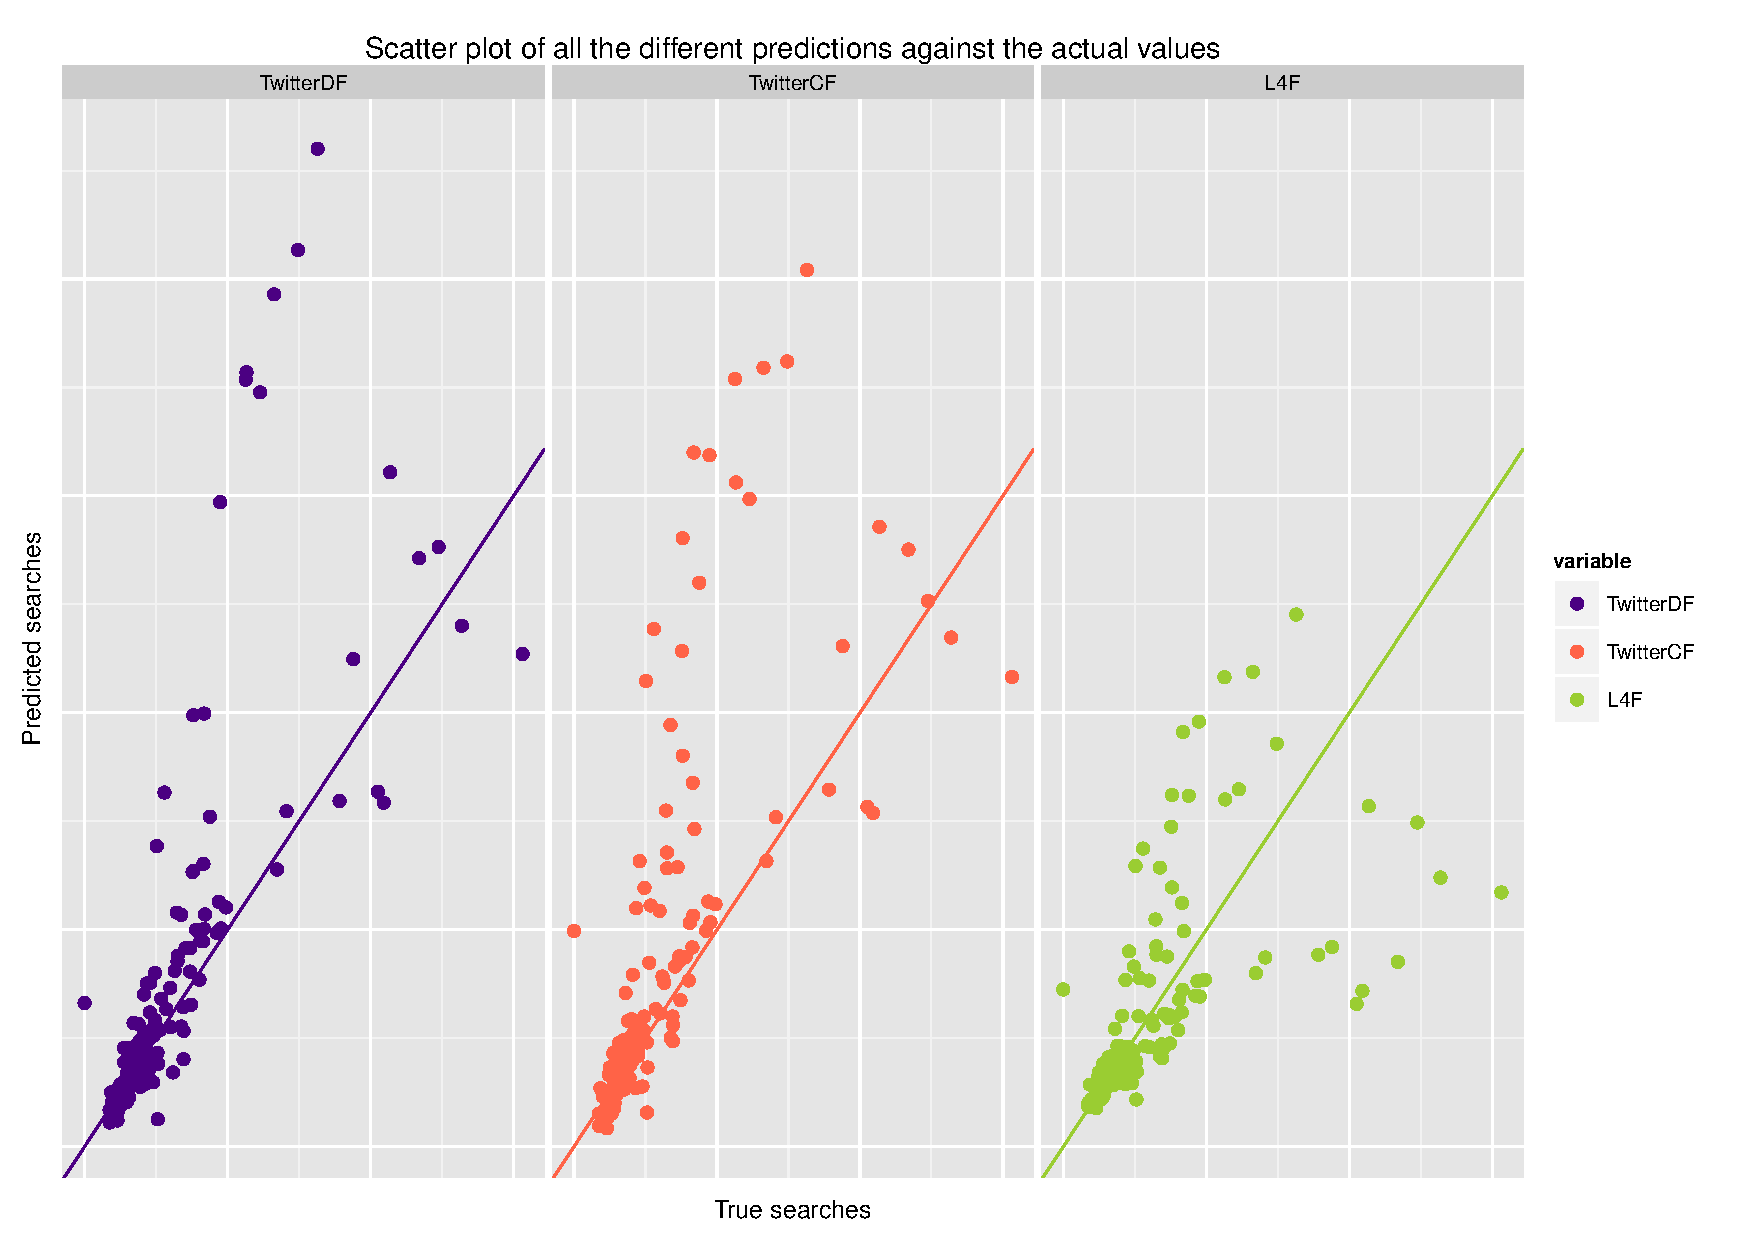
\includegraphics[scale=0.5]{plots/Sochi}
\end{center}
\caption{Predictions vs actual for a destination for Sochi. The olympics made any pattern in the data very hard to spot. The line $y = x$ is shown to portray the quality of the prediction.}
\end{figure}


\newpage
\subsection{UK}

The previous two examples showed that a for some destinations there is definitely an improvement by taking the expanded set of features, But also it not only improves the predictions, but by looking at the most prominent weights, we can infer some information on why these features are picked -- they can relate to events or could reflect on the socio-political situation. 

The United Kingdom is definitely not one of the destinations, where we see an improvement as shown in Table \ref{uk}.  Even though there is a very significant improvement in the RMSE as we increase the regularisation parameter it is still not enough to bear the baseline model. At $\alpha=32000$ there are still 14 and 11 weights in TwitterDF and TwitterCF. That means that if we wanted we could continue increasing the penalisation factor further, but that would turn tweaking and tuning the classifiers into a very complicated and laborious task and of course we will get into the problem of overfitting.

\begin{table}[h]
\begin{center}
\begin{tabular}{ l | r | r | r | r | r | r}
$\alpha$ & $>$ 0 W CF & MultiTwitterCF & $>$ 0 W DF & MultiTwitterDF & L4F & Best\\
\hline
0.5 & 583 & 60,924 & 649 & 70,068 & 8,700 & L4F\\
1 & 467 & 65,234 & 523 & 68,728 & 8,700 & L4F\\
2 & 369 & 65,253 & 412 & 76,945 & 8,700 & L4F\\
5 & 280 & 59,667 & 290 & 69,158 & 8,700 & L4F\\
10 & 231 & 54,972 & 241 & 62,057 & 8,700 & L4F\\
20 & 197 & 58,161 & 212 & 55,629 & 8,700 & L4F\\
50 & 167 & 62,001 & 175 & 77,956 & 8,700 & L4F\\
125 & 147 & 59,146 & 155 & 90,270 & 8,700 & L4F\\
250 & 139 & 73,864 & 142 & 105,197 & 8,700 & L4F\\
500 & 116 & 81,806 & 120 & 96,173 & 8,700 & L4F\\
1,000 & 106 & 84,796 & 110 & 91,576 & 8,700 & L4F\\
2,000 & 98 & 61,891 & 94 & 60,692 & 8,700 & L4F\\
4,000 & 71 & 44,306 & 68 & 61,037 & 8,700 & L4F\\
8,000 & 44 & 56,021 & 43 & 49,030 & 8,700 & L4F\\
16,000 & 27 & 31,209 & 29 & 28,339 & 8,700 & L4F\\
32,000 & 11 & 15,895 & 14 & 16,034 & 8,700 & L4F\\
\end{tabular}
\end{center}
\caption{Expanded features for the United Kingdom. We don't notice the same gain here. Both TwitterDF and CF decrease the number of features significantly the RMSE for both is about 2x times the one for L4F.}
\label{uk}
\end{table}

\newpage
\section{Results on the full dataset}

Another interesting benchmark was how it performs on the overall search volumes. In Table 4.11 you will find how the two models perform on the all the Twitter counts summed together and the searches to all of those destinations.

\begin{table}[h!]
\begin{center}
\begin{tabular}{ l | r | r | r | r}
 & TwitterDF & Twitter CF & L4F & Difference \\
\hline
Overall & 1,640,111 & 1,621,391  & 1,674,130 & 3.1 \% \\
\end{tabular}
\end{center}
\caption{RMSE on the tweet counts for all destinations and searches to all destinations. Difference is the percentage improvement of the best of the twitter models.}
\end{table}

As you can see in Figure \ref{overall-searches} the overall volume of searches is not as volatile as the destinations in group 2, so it would fall into group 1, but surprisingly enough the Twitter models do a marginally better job at predicting.

\begin{figure}[h]
\begin{center}
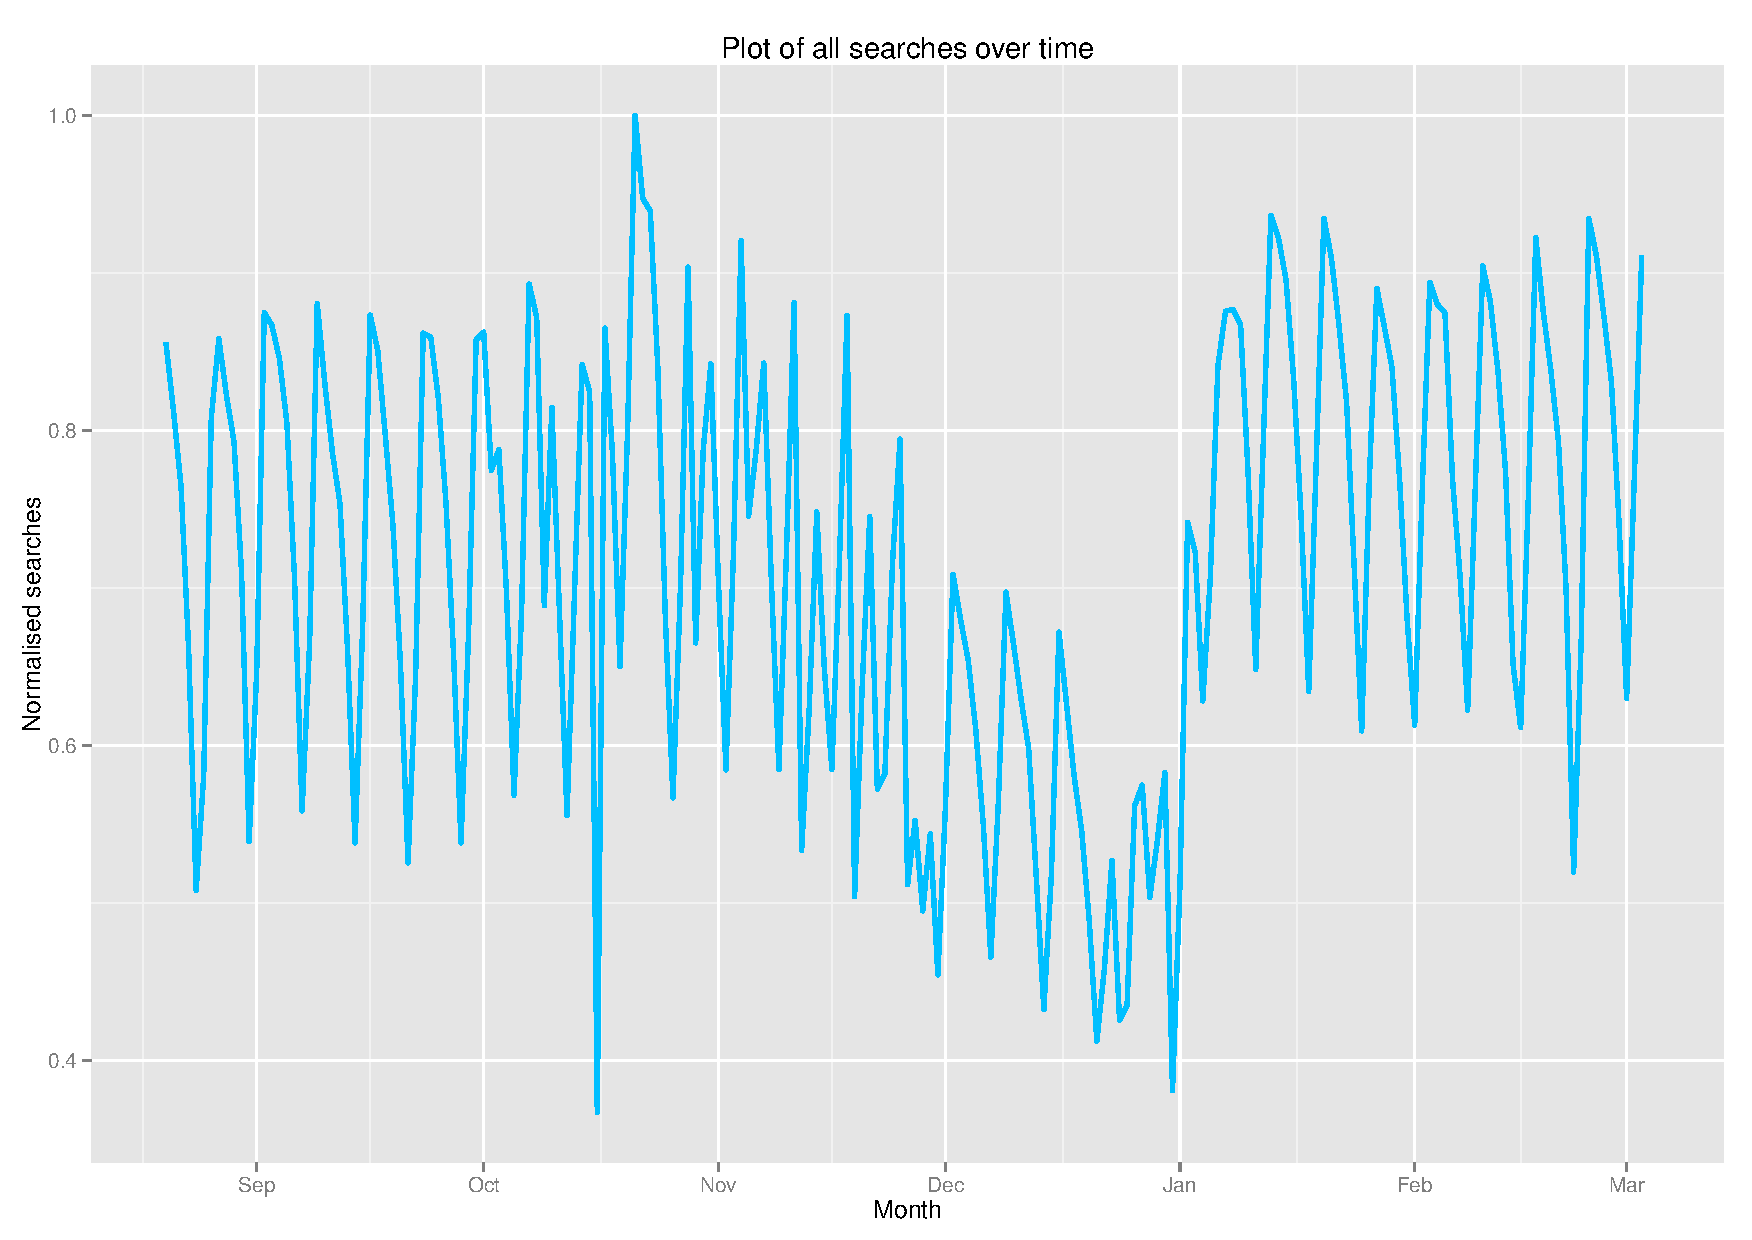
\includegraphics[scale=0.5]{overall}
\end{center}
\caption{Plot of all the searches to all the destinations. This would fall into the first group of steady constant volumes}
\label{overall-searches}
\end{figure}



\newpage
\section{Conclusion}

The previous results have demonstrated that there is definitely a gain, even though not as great as I expected, in including exogenous factors such as Twitter in the prediction. With the level of filtering described in Chapter \ref{sec:tweettext} on page \pageref{sec:tweettext} we have achieved better prediction on slightly more than 83\% of all the destinations.  


Overall he median decrease of RMSE for TwitterDF over the Last 4 Fridays is \textbf{4\%}. With TwitterCF the median improvement is \textbf{0.6\%} across all destinations. The TwitterCF improvement over L4F is \textbf{5\%}, which is very good. 


Even though it's not a double digit gain, it is still very significant. The fact that it was able to capture the recent events in Ukraine, Sochi and Venezuela and factor them in the predictions shows that using exogenous factors in your model for predicting search volumes is beneficial.


During the 2nd phase of the project, I will focus on retrieving only the most relevant tweets from the Twitter dataset and doing better feature extraction that will allow to remove junk features that bring the RMSE up. With that in mind, I am hopeful that I will be able to build the next version of the model that is going to perform just as well on the first group of destinations. 




\chapter{Future work}
\label{chap:future-work}

There has been a lot of work done for the first phase of the project, however I remain confident that there are many things I can work on and improve during the second phase. There are different avenues for future work to explore and in this chapter I outline the ones that are worth exploring.

\section{Applying more NLP and NLU}


My primary dataset is the 550 GB of Twitter data that I have accumulated since the 24th of September last year. The data contains 650 million tweets each containing up to 140 characters and that is a lot of text to work with. As we know NLP and NLU are the things which you apply on your text dataset.

In order to filter out my data I have so far used a simple method of filtering out the tweets and taking only the ones that have a certain name of a city/country and/or a word from the dictionary of travel-related terms shown in Figure 2.2. That worked very well, but it meant that I am not utilising this rich dataset to its fullest. 


The travel dictionary is one of the first points for improvement. The current list of words was picked after about 2 days of research. In order to improve the words in it, one could scrape some travel related websites for articles and figure out which are the words with highest TF-IDF scores in those documents. Then by picking the N most popular words we will end up with a new dictionary. With the new dictionary we can perform another filtering on the dataset. Then we can see which corpus yields the dataset with better correlation between the time series and the best search volume prediction.


The second point of improvement would be to use more advanced filtering of the incoming data from the Twitter Public Stream. The Streaming API has built-in the capability to track only specific words. Tracking only a certain set of words will reduce the data flowing in, but by doing this we are taking a risk of losing all the relevant tweets which our filters did not capture. This will be very important to work on, but is definitely not to be rushed.


The most interesting piece of NLP work that can be done with this dataset is to figure what the correlation of Twitter counts and search volumes would be without carrying out the Pearson test between the two. That means that by analysing the tweets for a particular we will be able to say whether taking Twitter will be beneficial and whether by taking it we will improve of reduce the quality of the prediction. The big scope makes this perhaps the most difficult task that I will work on next year. We will have to employ some advanced understanding of the tweets and figure what are the factors that drive the predictions up or down -- is it something in general or is it related only to certain events. In order to do that we will have to incorporate basic TDT with some Online Machine Learning to do that. With the data constantly flowing in I will be able to re-train the LASSO every hour or day in order to pick up the most interestings things that happened on the day and how they affected the search volumes. I plan to dedicate a significant portion of my time on the project next year in order to answer this difficult question, as I believe this will be the most beneficial thing that will improve the quality of the work,

With the system for correlation detection we will able to say exactly why Sochi had a correlation coefficient of 0.77 -- because of the Olympics -- and why Venezuela and Ukraine had -0.35 and -0.36. Of course as people who are aware of the current affairs, we know exactly why this is happening, but I will aim to build a system that will be able to give those on a daily basis. 


One way we can do that is to use LASSO again. We saw that LASSO gives us very interesting weights that are correlated to the events we have. In order to pull out the most interesting things for the day we will need to fit the LASSO on a daily or even an hourly basis so it can give us the most interesting and relevant things for the moment. 


For Sochi it gave us quite a few tags which pointed to the Olympics so we can easily see exactly why there is a massive upturn in demand for flights there. For Ukraine some of the features with high positive and negative weights were -- ``police'', ``protesters'', ``\#euromaidan''. Again for a human it is fairly easy to make the connection with the riots that were taking place. However how do you pull the most important ones in order to give a story? For this I might use additional data sources, which I will crawl in order to get the news stories. 


Having said all of the above, I strongly believe that NLP and NLU will give very interesting findings -- they can lead to understanding what makes people more or less likely to travel to a place and understand which events make a place more attractive. Quite a significant portion of my time next year will be spent on working and improving those systems. 


\section{More advanced ML methods}


The next possible avenue for improvement is of course trying more advanced ML methods to improve the prediction of search volumes. 

Common ``trick" in the ML community is to use LASSO for the feature selection and to pick the weights for the individual features, which are then passed on to a Ridge regression model to do the actual classification. As mentioned in Chapter 3.6, I have tried that in this phase of the project, but the results yielded were exactly the same as the ones produced by LASSO, with the difference being about 3 digits after the percentage point. Therefore the overall effect was minimaI. 


I have also trained a Ridge regression with its own learned coefficients and that did produce some small incremental improvements, but it did not change the balance of overall picture - the ones predicted better by L4F were still predicted better by it and there was a very small improvement for the ones where the Ridge regression was better. I believe the benefits of the bigger penalisation of the Ridge regression model will benefit more the MultiFeatureTwitter models where we have loads of features. The higher penalty will hopefully bring the RMSE down. Hence this is one of the first thing I will try in the second phase of the project. 


I have mentioned in the previous section, that I will try to do some more advanced feature selection to determine which words should be tracked and which not. There are various algorithms that could be tried to do this particular job and with the past data I will determine the most relevant words, so I can track only the ones that maximise my changes of receiving only the most relevant tweets. 


Of course there are a few more algorithms that I need to try -- Bayesian Ridge Regression, Elastic Net and Multi-Task Lasso. It will be interesting to try all of those, because even though they belong to the same family of linear models they should yield very different results, which will have to be discussed. 


The TDT work described in the previous section will only benefit from an online machine learning system capable of updating its weights, re-fitting and producing forecasts in real time. When an event is flagged as potentially something that affects searches, the online ML system will kick in, train a model and make a prediction. After receiving the actual data, it will factor those in and continue improving itself.



\section{More sophisticated method for data processing}


With the rise of ``Big Data" there are now numerous ways and tools for working with very big datasets. Perhaps the most popular tool for dealing with big volumes of data nowadays is Hadoop. It uses a network of commodity hardware computers to parallelise computation in an efficient way. I didn't use Hadoop, because the volumes were not that great, so it was still possible to work with the with my own scripts. 


Having just gone past 550 GB of data and 650 million tweets, it's now very time-consuming to do any in-depth analyses on the dataset. In order to carry out the NLP and NLU work described in Chapter 5.1 I will need a very robust platform for data processing that will not buckle under the terabyte load of data. I plan on asking the School of Informatics for some disc space and permission to use the Hadoop cluster in order to perform all the heavy lifting for my dissertation in Hadoop. This way I will be able to do all of the Twitter processing and aggregation on the cluster and not on my machine. I believe that by employing the parallel power of Map Reduce I will be able to aggregate a few additional cuts of data and that I will be finally able to perform feature extraction at scale -- something that I am not able to do currently because of hardware limitations. 


\section{Applications at Skyscanner}


Since this project was done in conjunction with Skyscanner, let's examine what impact it will have on the company. 
They will be able to use this to predict search volumes straight away. By having a look at which destinations benefit, they can start collecting data on a daily basis, aggregating and throwing away the unneeded dataset. By doing this they will be able to improve their prediction by more than 5\%. As the company grows, the need for more accurate and more versatile and robust prediction will become greater. Hence why the company will benefit from using this method of predicting flight search volumes with exogenous factors. 


It has been briefly touched on in previous sections, but using the LASSO weights for the features could tell a story -- what exactly happened in the past X days or hours. By re-training the models for every place you can pick out the most interesting features and those on their own can tell a good story of what has influenced people. Of course, that can also be used on historical data to classify any present spikes and create a narrative of what influences people's decisions and what exactly makes them want to buy a plane ticket. 

\section{Outline for the second phase}

Here is the outline for next year:

\begin{itemize}
\item Ask for permission to use the Hadoop cluster. If given, migrate the data to it and write the MR jobs that crunch the data. 
\item Extract the features and work on the MultiTwitterFeature Ridge models. I expect this to take a couple of week at most. 
\item Improve the dictionary by using LDA or other topic models in order to pick the most relevant words connect to travelling. After finishing this, re-filter the data and obtain the new working data set. Do all the work from phase 1 and obtain the new results. If results are better go with the new one. This work should be done by mid-November
\item Start working on the correlation system that will explain which places will have a good correlation and which not. I hope this will be done by end of January. 
\item After working on the correlation system start drafting out the real time system with online machine learning. This will be quite a good piece but it will produce a lot of interesting statistics. This will take until the end of February or mid-March.
\item While working on the real time system implement all the other ML algorithms mentioned above. Benchmark and evaluate them both with the real time system and with the non-real time one -- beginning of March.
\item Draft done by middle March and final version done a week before. 
\end{itemize}



\section{Conclusion}


There has been a lot of work during the first phase of this project. I have connected two datasets who haven't been done so before; Skyscanner can already use this for prediction and I have beaten the prediction by 5\%. The multi feature models have laid the ground work for a more complicated system that can give the most interesting things mentioned on Twitter and therefore the most interesting things that happened and were tweeted about. 


With all of that taken into account there is still a lot left to do. I remain confident that by following the plan I will stay on track on produce a cutting-edge system for social media analytics, that can be easily plugged in to aid prediction of any metric. It will not just predict, but also give context on why the predictions are the way they are -- X happened and that increased the volume for that place by Y\%. 


It is a very ambitious goal, but with the right help, mentoring and careful planning I am positive that the end result will be a system designed in such a way that it can be easily used by anyone. And it's not just used, it's also useful and does what promised.


\raggedright
%\sloppy
\bibliographystyle{unsrt}
\bibliography{master}

\end{document}
